\chapter{The LEGEND experiment}
\label{ch:legend}

The Large Enriched Germanium Experiment for Neutrinoless double beta Decay (LEGEND) is a multi-phase experimental program searching for the $0\nu\beta\beta$ decay of ${}^{76}$Ge. Located deep underground at the Gran Sasso National Laboratories (LNGS) in Italy, under a rock overburden of approximately 3500 m.w.e. (meter water equivalent), LEGEND operates in an environment heavily shielded from cosmic radiation.

The experiment is designed to operate in two distinct phases. In its first stage, LEGEND-200, it is currently operating with roughly 200 kg of enriched germanium detectors. Its objective is to achieve a background index of $2 \times 10^{-4}$ cts/(keV$\cdot$kg$\cdot$yr) to reach a discovery sensitivity greater than $10^{27}$ yr with 1 t$\cdot$yr of exposure. The subsequent phase, LEGEND-1000, will scale the target mass up to 1000 kg, aiming for an unprecedented background goal of $1 \times 10^{-5}$ cts/(keV$\cdot$kg$\cdot$yr) to reach a sensitivity greater than $10^{28}$ yr with an exposure of 10 t$\cdot$yr.

To achieve such ambitious goals, LEGEND builds upon the successful technologies and background mitigation strategies developed by its predecessors, the GERDA and \textsc{Majorana Demonstrator} experiments. By utilizing \ac{hpge} detectors enriched in ${}^{76}$Ge, the experiment benefits from the \textit{source-equals-detector} approach. This maximizes the detection efficiency and exploits the outstanding energy resolution of semiconductor detectors to clearly separate the mono-energetic $0\nu\beta\beta$ signal from the $2\nu\beta\beta$ irreducible continuous background.

Reaching the required ultra-low background regime demands a multi-layered active and passive shielding strategy. This is accomplished by operating the bare germanium array directly in an instrumented Liquid Argon (\ac{lar}) cryostat, surrounded by a \ac{lar}ge water Cherenkov veto, and by employing sophisticated signal processing techniques to reject localized background events. The following sections detail the experimental apparatus and the event selection methods crucial to the experiment success. \cite{LEGEND:GeDet}

\section{Experimental setup}
\label{sec:expsetup}
The experimental setup of the LEGEND program builds upon the decommissioned GERDA experiment. It repurposes GERDA infrastructure and inherits its shielding concept, which relies on a low-Z shield (water and argon) and an active veto system based on the detection of scintillation light. \cite{LEGEND:introSetup}

The whole structure of the setup is shown in Figure~\ref{fig:L200setup} and consists of:
\begin{itemize}
    \item slightly less than 200 kg of \ac{hpge} detectors;
    \item a \ac{lar} cryostat;
    \item a water tank for Cherenkov light detection.
\end{itemize}

\begin{figure}[H]
    \centering
    % Immagine a sinistra
    \begin{minipage}{0.55\textwidth}
        \centering
        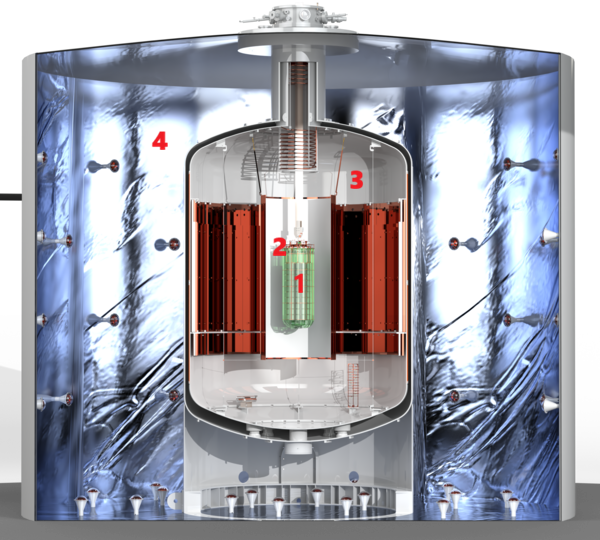
\includegraphics[width=\linewidth]{figures/LEGENDwholeSetup_con-numeri.png}
    \end{minipage}\hfill
    % Immagine a destra
    \begin{minipage}{0.40\textwidth}
        \centering
        % SOSTITUISCI IL NOME DEL FILE QUI SOTTO
        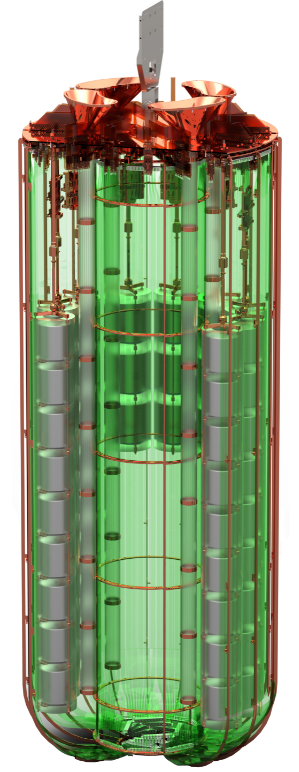
\includegraphics[width=0.5\linewidth]{figures/LEGENDLAr.png}
    \end{minipage}
    
    \caption{On the left, the whole experimental setup for the LEGEND-200 phase: the picture shows the \ac{hpge} detectors (1), the \ac{lar} instrumentation (2), the \ac{lar} cryostat (3) and the water tank provided with the Cherenkov detectors (4). On the right, a close-up of the \ac{lar} instrumentation where the detector strings are visible. Rendering by P. Krause, taken from \cite{LEGEND:setup}.}
    \label{fig:L200setup}
\end{figure}

\subsection{Germanium detectors}
\label{subsec:GeDetectors}
The \ac{hpge} detectors are semiconductor diodes sensitive to ionizing radiation and $\gamma$-rays. They provide excellent energy resolution and high detection efficiency, acting as both the source and detector for double-beta decay. 

LEGEND-200 utilizes 142.5~kg of p-type \ac{hpge} detectors arranged in vertical strings. Four detector types are deployed: 
\begin{itemize}
    \item 86.7~kg of \ac{IC} detectors newly designed and produced for LEGEND (41 detectors),
    \item 22.1~kg of p-type Point-Contact (PPC) detectors from \textsc{MAJORANA DEMOSNTRATOR} (26 detectors),
    \item 19.0~kg of Broad Energy Germanium (BEGe) detectors from GERDA (28 detectors),
    \item 14.7~kg of semicoaxial (Coax) detectors also from GERDA (6 detectors).  
\end{itemize}
Typical individual detector masses are $1$~kg for PPC, $2.5$~kg for Coax, $0.7$~kg for BEGe, and $2-4$~kg for IC. Said detectors are enriched in $^{76}$Ge up to 86--92\%, depending on the detector type. The geometry of all of the detectors is shown in Fig. \ref{fig:detectors-types}. The \ac{IC} detectors, comprising the largest fraction of the array, feature the most advanced design in terms of sensitivity to $0\nu\beta\beta$ decay, combining high energy resolution and large individual masses to effectively reduce the background level. \cite{articoloSaleh}

\begin{figure}[ht]
    \centering
    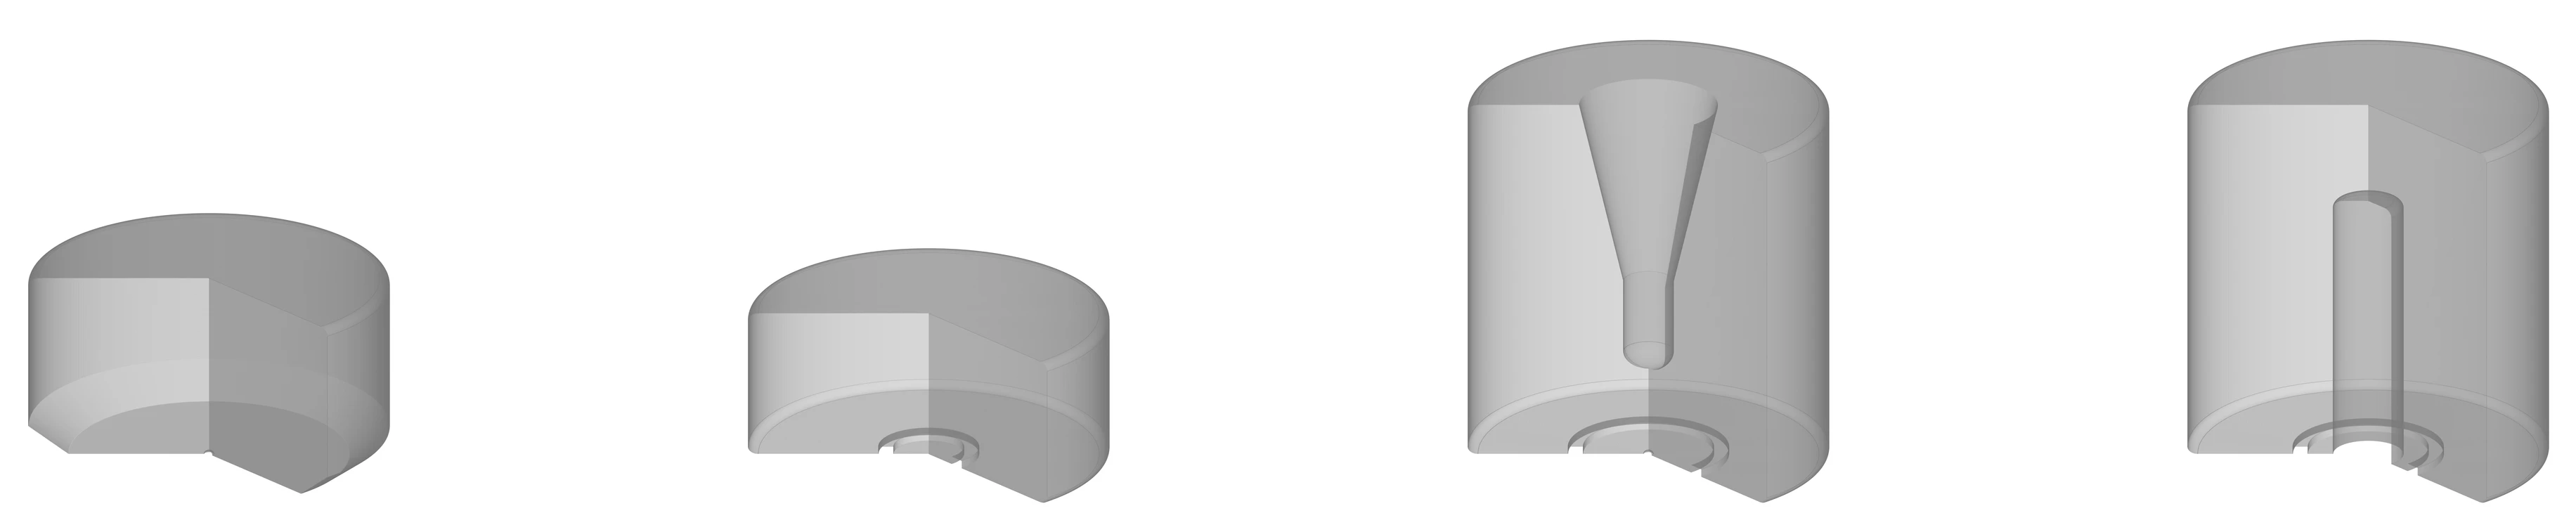
\includegraphics[width=\textwidth]{figures/4Detectors.png}
    \caption{Drawing of the different Germanium detectors employed in LEGEND. From the left to the right: PPC, BEGe, Coax and IC detectors respectively. Rendering by D. Hervas.}
    \label{fig:detectors-types}
\end{figure}

The \ac{hpge} detectors operate with a reverse bias voltage, which depletes almost the entire volume of free charge carriers. A \ac{HV} up to 5~kV is applied to the $n^+$ electrode, which features a relatively thick ($\sim 0.7$~mm) Li-diffused dead layer, while the signal is readout from the thin ($\sim 0.3$~$\mu$m) $p^+$ electrode, created via boron implantation.

These detectors are mounted on supports made of active PolyEthylene Naphthalate (PEN), a scintillating plastic material known for its ability to improve background rejection. To maintain high radiopurity near the detector array, low-mass Majorana components and underground electroformed copper are used to reduce the effects of ${}^{238}$U and~${}^{232}$Th decay chains and cosmogenic activation of~${}^{60}$Co in copper. Each \ac{hpge} string is enclosed in a TPB-coated nylon cylinder, called Nylon Mini Shroud (NMS), to minimize the \ac{lar} volume around the detectors, preventing the capture of radioactive ions like~${}^{42}$K by electric fields on the detector surfaces\footnote{See Sec \ref{sec:background} for further details on these background strategies.}. \cite{LEGENDsetup-details}

The detectors and liquid argon instrumentation are assembled in the clean room above the cryostat in a glove box which is flushed with nitrogen to avoid, or at least reduce, Radon deposition on the detectors and protects the insulating groove between the detector $p^+$ and $n^+$ electrodes by an inert atmosphere. \cite{LEGEND:setup}

\subsection{Liquid Argon cryostat}
\label{subsec:LAR}
A 4~m-diameter vacuum-insulated stainless steel cryostat with 64~m$^3$ of purified Liquid Argon (\ac{lar}) is present. The ultra-pure \ac{lar} acts as a cooling medium for the germanium detectors and as a shield for external radiation. At the bottom of the cryostat, the LEGEND \ac{lar} Monitoring Apparatus (LLAMA) is placed, allowing to monitor the purification levels of the \ac{lar} continuously.

The center of the cryostat contains a 1374~mm-diameter and 3~m-height cylinder, made of copper-tetratex foil coated internally with TetraPhenyl Butadiene (TPB), called WaveLength-Shifting Reflector (WLSR). The WLSR is designed to separate the innermost \ac{lar} volume (about 6~t of \ac{lar}), working as further shielding for detector systems and as a reflector of the \ac{lar} scintillation light.

The \ac{lar} instrumentation is located within the WLSR and consists of two concentric WaveLength-Shifting (WLS) fiber shrouds that surround the germanium detectors (Fig. \ref{fig:L200setup} right). The WLS fibers are coupled to \ac{SiPMs} at both ends. The \ac{lar} instrumentation is crucial for detecting background events that deposit energy in the \ac{lar} volume surrounding the germanium detectors. \cite{LEGENDsetup-details}

% The cryogenic infrastructure of the cryostat includes the liquid argon and nitrogen storage tanks, a valve box which houses manual and remotely controlled valves for LN$_2$/\ac{lar} and a radon trap, and piping inside the cryostat. The latter includes two copper spirals as heat exchangers for the cooling of \ac{lar} with LN$_2$, a \ac{lar} filling line, a drainage pipe, temperature sensors at different positions, and several devices for the fill level measurement. The available aperture for the detectors in the neck is reduced because of these pipes and sensors such that this opening becomes the limiting cross section. For LEGEND-200, the installation has been replaced to enlarge the area for detectors and \ac{lar} instrumentation. \cite{LEGEND:setup}

\subsection{Water tank}
A 10~m-diameter and 8~m-height tank with 590~m$^3$ of ultra-pure water shields from neutron and gamma backgrounds. It works also as a muon veto for residual cosmic muons through the detection of Cherenkov light with 63 \ac{PMT} (8” size) of type 9354KB/9350KB by ETL. In order
to protect the \ac{PMT} from the surrounding water, each PMT is housed in a stainless-steel encapsulation which is further developed from the design of the Borexino capsules. The \ac{PMT} are arranged in seven rings in the water tank. One ring of six \ac{PMT} is pointing inside the separate volume under the cryostat,  two rings of eight \ac{PMT} and 12 \ac{PMT}  respectively are placed on the bottom of the water tank looking upwards and four rings of 10 \ac{PMT} are placed on the wall, pointing horizontally towards the cryostat. \cite{GERDA-muonVeto} 



\newpage
\section{Background contaminations}
\label{sec:background}
Background is one of the main issues in the LEGEND program. According to \cite{L200-sep25} the background contribution for the LEGEND experiment are the same of its predecessor GERDA, therefore further consideration about it are based on \cite{GERDAphase2}.

% The spectrum is dominated by the $\beta$ decay of ${}^{39}$Ar in the \ac{lar} up to 565 keV, while the $2\nu\beta\beta$ decay of ${}^{76}$Ge becomes the prominent component between 600 keV and 1500 keV. Additionally, two $\gamma$ lines at 1461 keV and 1525 keV originate from ${}^{40}$K and ${}^{42}$K, respectively, with other spectral lines attributed to ${}^{58}$Kr, ${}^{208}$Tl, ${}^{212}$Bi, and ${}^{228}$Ac. At higher energies, the $\alpha$ decay of ${}^{210}$Po leaves a distinct signature at 5.3 MeV, and the peaks emerging above this energy are driven by $\alpha$ decays within the ${}^{226}$Ra decay chain. 

The main contribuitions to background are:
\begin{itemize}
    \item \textbf{${}^{238}$U and ${}^{232}$Th decay chains}:\\
            The radioactive isotopes to be considered are ${}^{234\text{m}}$Pa\footnote{The m stands for metastable.}, ${}^{214}$Pb and ${}^{214}$Bi from the ${}^{238}$U chain and ${}^{228}$Ac, ${}^{212}$Bi and ${}^{208}$Tl from ${}^{232}$Th. Their products are $\gamma$ rays or $\beta$ particles with an energy higher than 520 keV\footnote{Higher energies are not taken into cosnideration because are outside of the energy window of interest.}. If any $\alpha$ particle is produced, it is considered as described in the following points
    \item \textbf{${}^{60}$Co}:\\
            A significant part of the \ac{hpge} infrastructure is made up of copper (see Sec \ref{subsec:GeDetectors}) that can be produced in safe enviroments avoiding contaminations, but can be nevertheless be activated by cosmic rays that may produce the long-lived isotope ${}^{60}$Co ($\tau_{1/2}^{{}^{60}\text{Co}} = 5.2711(8)$ yr). Furthermore, also \ac{HV} copper cables can have a small component of such isotope.

    \item \textbf{${}^{40}$K:}\\
            This specific isotope is present in all of the screened materials, seeing that the Q-value of its decay is well below the enrgy region of interest and therefore does not contribute with background around $Q_{\beta\beta}$.

    \item \textbf{${}^{42}$K:}\\
            In liquid argon (\ac{lar}), one of the primary cosmogenically produced isotopes is ${}^{42}\text{Ar}$ ($\tau_{1/2} = 32.9(11)\text{ yr}$), which decays into ${}^{42}\text{K}$. The spatial distribution of this potassium isotope inside the \ac{lar} tank is expected to be inhomogeneous due to the drift of ionized decay products—induced by the electric field generated by high-voltage cables and detectors—as well as fluid convection. ${}^{42}\text{K}$ subsequently undergoes $\beta$ decay to ${}^{42}\text{Ca}$ with a half-life of $\tau_{1/2} = 12.355(7)\text{ h}$ and a Q-value of $3525.22(18)\text{ keV}$, which lies well above $Q_{\beta\beta}$. 
            For a $\beta$ particle to be directly detected, the decay must occur within a few centimeters of the detector surfaces; otherwise, the electrons are fully absorbed by the surrounding \ac{lar}. Because the detectors are in direct contact with the liquid argon, this $\beta$ component represents one of the most significant background contributions. A higher concentration of ${}^{42}\text{K}$ events is typically observed near the front-end electronics. Away from the electronics, the proximity of the decay to the detector outer contacts ($n^+$ and $p^+$) dictates the $\beta$ acceptance rate: the closer the decay happens to the surface, the higher the probability that $\beta$ particles enter the germanium volume. 
            Furthermore, a fraction of background events near $Q_{\beta\beta}$ originating from ${}^{42}\text{K}$ can be attributed to high-energy $\gamma$ rays with sub-percent branching ratios or to simultaneous multiple $\gamma$ depositions. This $\gamma$-induced component becomes particularly relevant when large quantities of ${}^{42}\text{K}$ are located further away from the detector surfaces, where direct $\beta$ particles are completely shielded and absorbed by the \ac{lar}.

    \item \textbf{$\alpha$ emitters:}\\
            The lithium-diffused $n^+$ detector surfaces act as a barrier for external $\alpha$ particles that as a consequence can only penetrate the detctor throught the $p^+$ surface. However, having to traverse the $0.5~\mu$m thick $p^+$ dead layer, said particles loose energy and their contribution to the background is relatively negligible. Some $\alpha$ events may arise from fabbrication contaminants onto the detector such as ${}^{210}$Po and ${}^{210}$Pb: having energies up to 5 MeV they can penetrate the detector surface and contribute to the continuous background.

\item \textbf{Detector bulk impurities:}\\
            Cosmogenically produced long-lived isotopes can act as intrinsic impurities within the Germanium crystals. In particular, ${}^{68}$Ge and ${}^{60}$Co can be produced if the detectors are exposed to cosmic radiation above ground during fabrication and characterization operations. However, based on background simulations from the GERDA project, the contribution of these bulk impurities around the $Q_{\beta\beta}$ value is expected to be less than $10^{-4}$ cts/(\text{keV}$\cdot$\text{kg}$\cdot$\text{yr}). Consequently, the background induced by these two isotopes is considered negligible.

    \item \textbf{Cosmic muons:}\\
            Prompt background events induced by cosmic muons are efficiently vetoed by identifying the Cherenkov light produced as they pass through the water tank, which is read out by the \ac{PMT} system. Furthermore, the expected background indices (BIs) due to direct muon and neutron fluxes at the LNGS underground laboratory are estimated to be extremely low, on the order of $3 \times 10^{-5}$ cts/(\text{keV}$\cdot$\text{kg}$\cdot$\text{yr}) and $10^{-5}$ cts/(\text{keV}$\cdot$\text{kg}$\cdot$\text{yr}), respectively. Cosmic muons can also induce delayed decays of ${}^{77}$Ge and ${}^{77\text{m}}$Ge, yielding a BI of about $10^{-5}$ cts/(\text{keV}$\cdot$\text{kg}$\cdot$\text{yr}) even prior to applying active suppression techniques. Given these exceptionally low values, all these muon-induced sources are deemed negligible.
            
    \item \textbf{Other sources:}\\
            Additional potential background contributions include contaminations in the water tank and the \ac{lar} cryostat, which are expected to yield a BI of less than $10^{-4}$ cts/(\text{keV}$\cdot$\text{kg}$\cdot$\text{yr}). Interactions of ${}^{76}$Ge and ${}^{206}$Pb with neutrons and ${}^{56}$Co are not taken into consideration, as no evidence for them was found. Finally, particles emitted by the cosmogenically produced ${}^{39}$Ar and the anthropogenic ${}^{85}$Kr, both dissolved in \ac{lar}, possess energies that are dominantly lower than the analysis window. Therefore, all these potential contaminations can be safely neglected in the region of interest.

\end{itemize}

As mentioned above, background signals are a complicated part to deal with in the LEGEND experiment and therefore every single part of it has been built considering that background sources have to be limited as much as possible. This is the reason why structural components of the setup have been screened for their radio-purity before deployment. In order to achieve this goal two methods depending on the screened isotope:
\begin{itemize}
    \item $\gamma$ ray spectroscopy (Ge-$\gamma$) with High Purity Germanium 
    \item mass spectroscopy with Inductively Coupled Plasma Mass Spectrometers (ICP-MS)
\end{itemize}

All of the materials close to the detectors have been screened to prevent radioactive contamination given by ${}^{238}$U and ${}^{232}$Th decay chains and ${}^{40}$K and ${}^{60}$Co isotopes.


\newpage
\section{LEGEND data}
\subsection{Detector physics and signal formation}
As already introduced in Sec. \ref{sec:expsetup}, experimental data of the LEGEND program rely on different types of detectors including \ac{hpge} detectors (acting also as the primary source for double-beta decay), scintillating fibers and SiPM for the \ac{lar} scintillation light and PMT tubes for muon-induced Cherenkov light. In this section \ac{hpge} detectors will be analysed in order to understand how signals are originated, collected, readout, processed and analysed in the LEGEND program. This is essential in order to lay the basis for the main focus of the thesis in Chapter \ref{chapter:ML-PSD}.

\paragraph{Germanium detectors basics}
\label{par:Ge-detector-basics}
%  \begin{wrapfigure}{r}{0.52\textwidth}
%   \centering
%   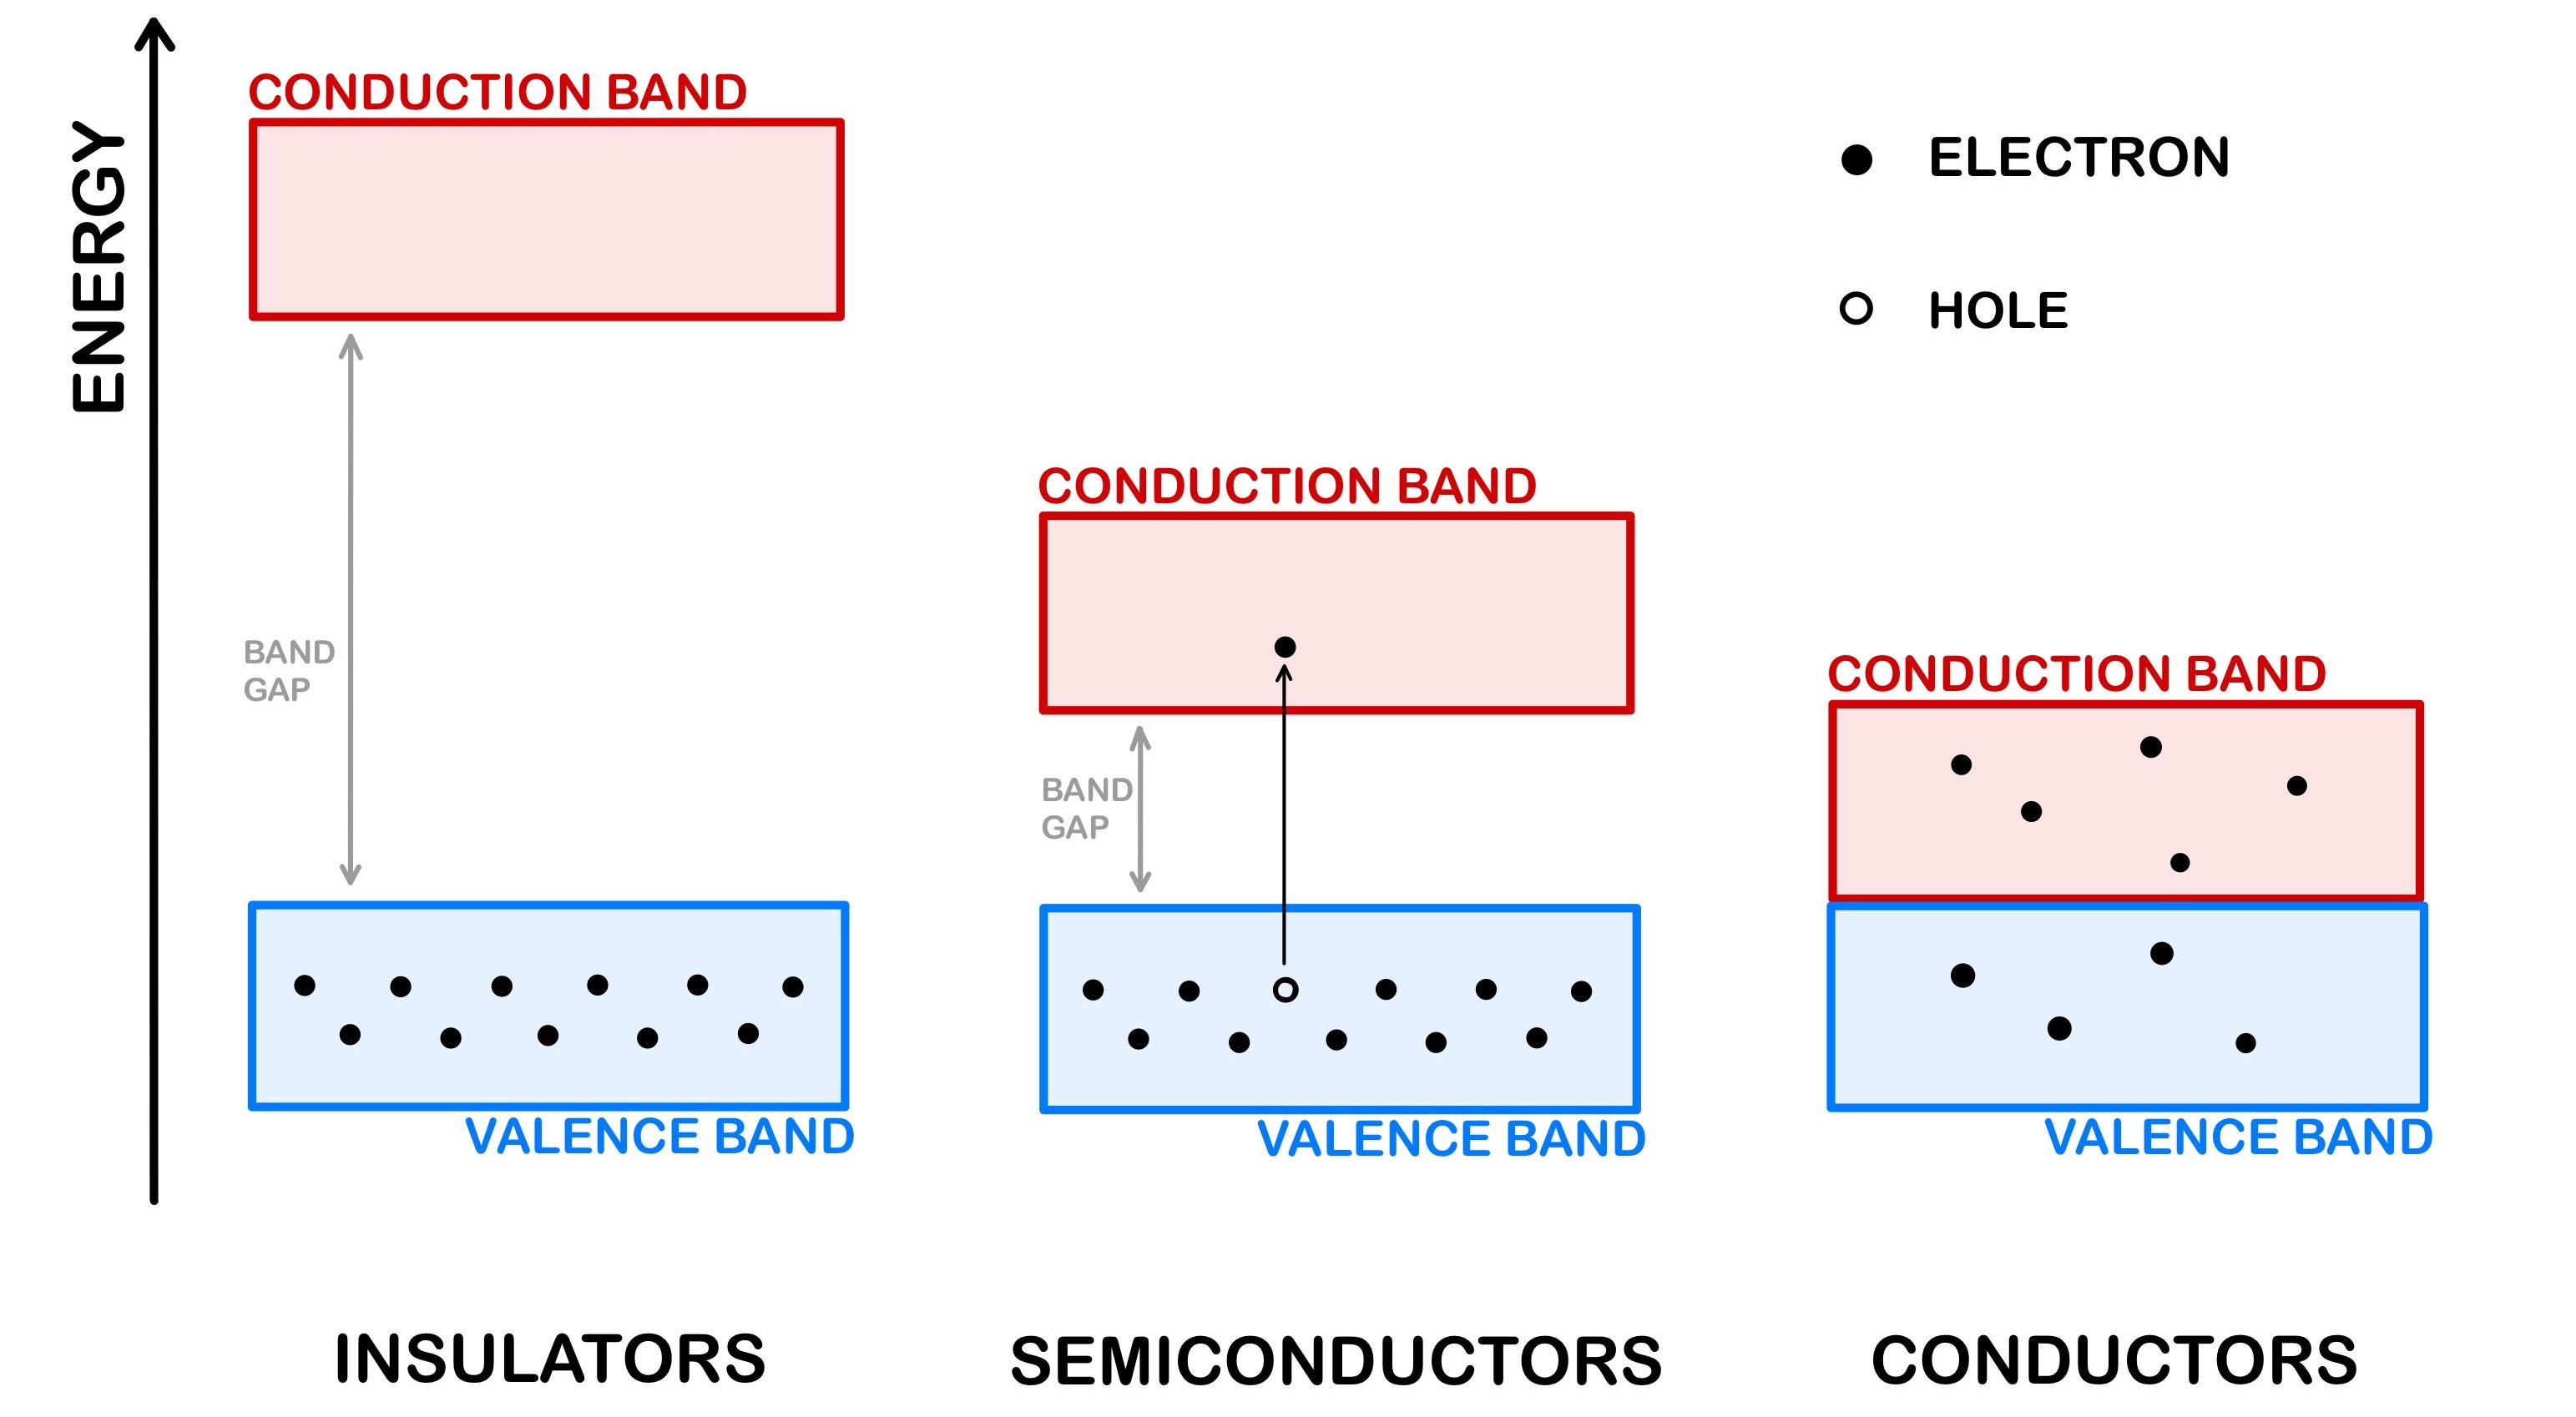
\includegraphics[width=\linewidth]{figures/insulators-semiconductors-conductors.jpg}
%   \caption{Energy levels and band gaps. From the left: insulators, semiconductors and conductors. Original drawing.}
%   \label{fig:band_gaps}
% \end{wrapfigure}
\ac{hpge} detectors are semiconductor detectors, therefore it is crucial to analyse some specific features of semiconductor materials.
Said materials are characterised by the typical crystalline diamond lattice where each Germanium atom is bonded to four nearest neighbours arranged in the corners of a regular tetrahedron. As a consequence of the dense periodic arrangement of the atoms in a solid-state lattice the energy levels of individual atoms are split due to the influence of many neighbouring atoms nearby. Seeing that energy levels of some level groups lie energetically very dense, we talk about \textit{energy levels} divided by \textit{band gaps}.
The two highest energy levels are called the valence band and the conduction band. Within a band, energy levels are so dense that transitions to unoccupied levels are very easy if the band is not completely filled. Therefore conduction properties depend on the band occupation. In semiconductor materials the bonds between neighbour atoms are weaker than the ones of insulators and this leads to smaller energy gaps. This becomes significant when we consider the energy gap between valence band and conduction band, since the energy gap can be overcome via thermal excitations or external electric fields: when a bond is broken, an \ac{eh} pair is generated. While the hole remains in the valence band, the electron can move freely to the conduction band. If this happens in an electric field, the moving charge generates a current flow. The energy gap between bands depends on the lattice spacing, which means that temperature and pressure influence the gap size $\text{E}_\text{G}$.
The relatively small band gap of germanium ($E_G \simeq 0.67$~eV at room temperature, compared to $1.12$~eV in silicon) has a direct consequence on the operating conditions of the detector. At $T = 300$~K the thermal energy is sufficient to promote a non-negligible number of electrons across the gap, yielding an intrinsic carrier concentration of the order of $10^{13}$~cm$^{-3}$. Once a bias voltage is applied, these thermally generated carriers are collected by the electrodes and give rise to a leakage current whose statistical fluctuations would completely overwhelm the charge released by a single ionising event. For this reason, HPGe detectors must be operated at cryogenic temperatures, where thermal generation is exponentially suppressed and the leakage current becomes negligible. In LEGEND this requirement is fulfilled by operating the bare detectors directly immersed in liquid argon at $\sim 87$~K, which therefore acts simultaneously as a cooling medium and as a shielding against external radiation (see Sec.~\ref{subsec:LAR}).

An artificial introduction of impurities in the semiconductor lattice can selectively change its behaviour in terms of conductivity.
Pentavalent elements called \textit{donors}, like Phosphorus, inserted in a tetravalent semiconductor like Germanium produce an excess of conduction electrons with respect to the holes; this is called \textit{n-doping}. On the other hand, \textit{p-doping} consists of placing in the lattice trivalent atoms called \textit{acceptors}, like Boron, leading to an excess of holes. The overall crystal of the semiconductor remains electrically neutral, because donors and acceptors are nevertheless neutral atoms, but the available number of charge carriers, either holes or electrons, changes leading to a modification in the conduction properties of the semiconductor. Pure semiconductors are called intrinsic semiconductors, while doped semiconductors are called extrinsic semiconductors. \cite{libro-detectors}
% \begin{figure}[H]
%     \centering
%     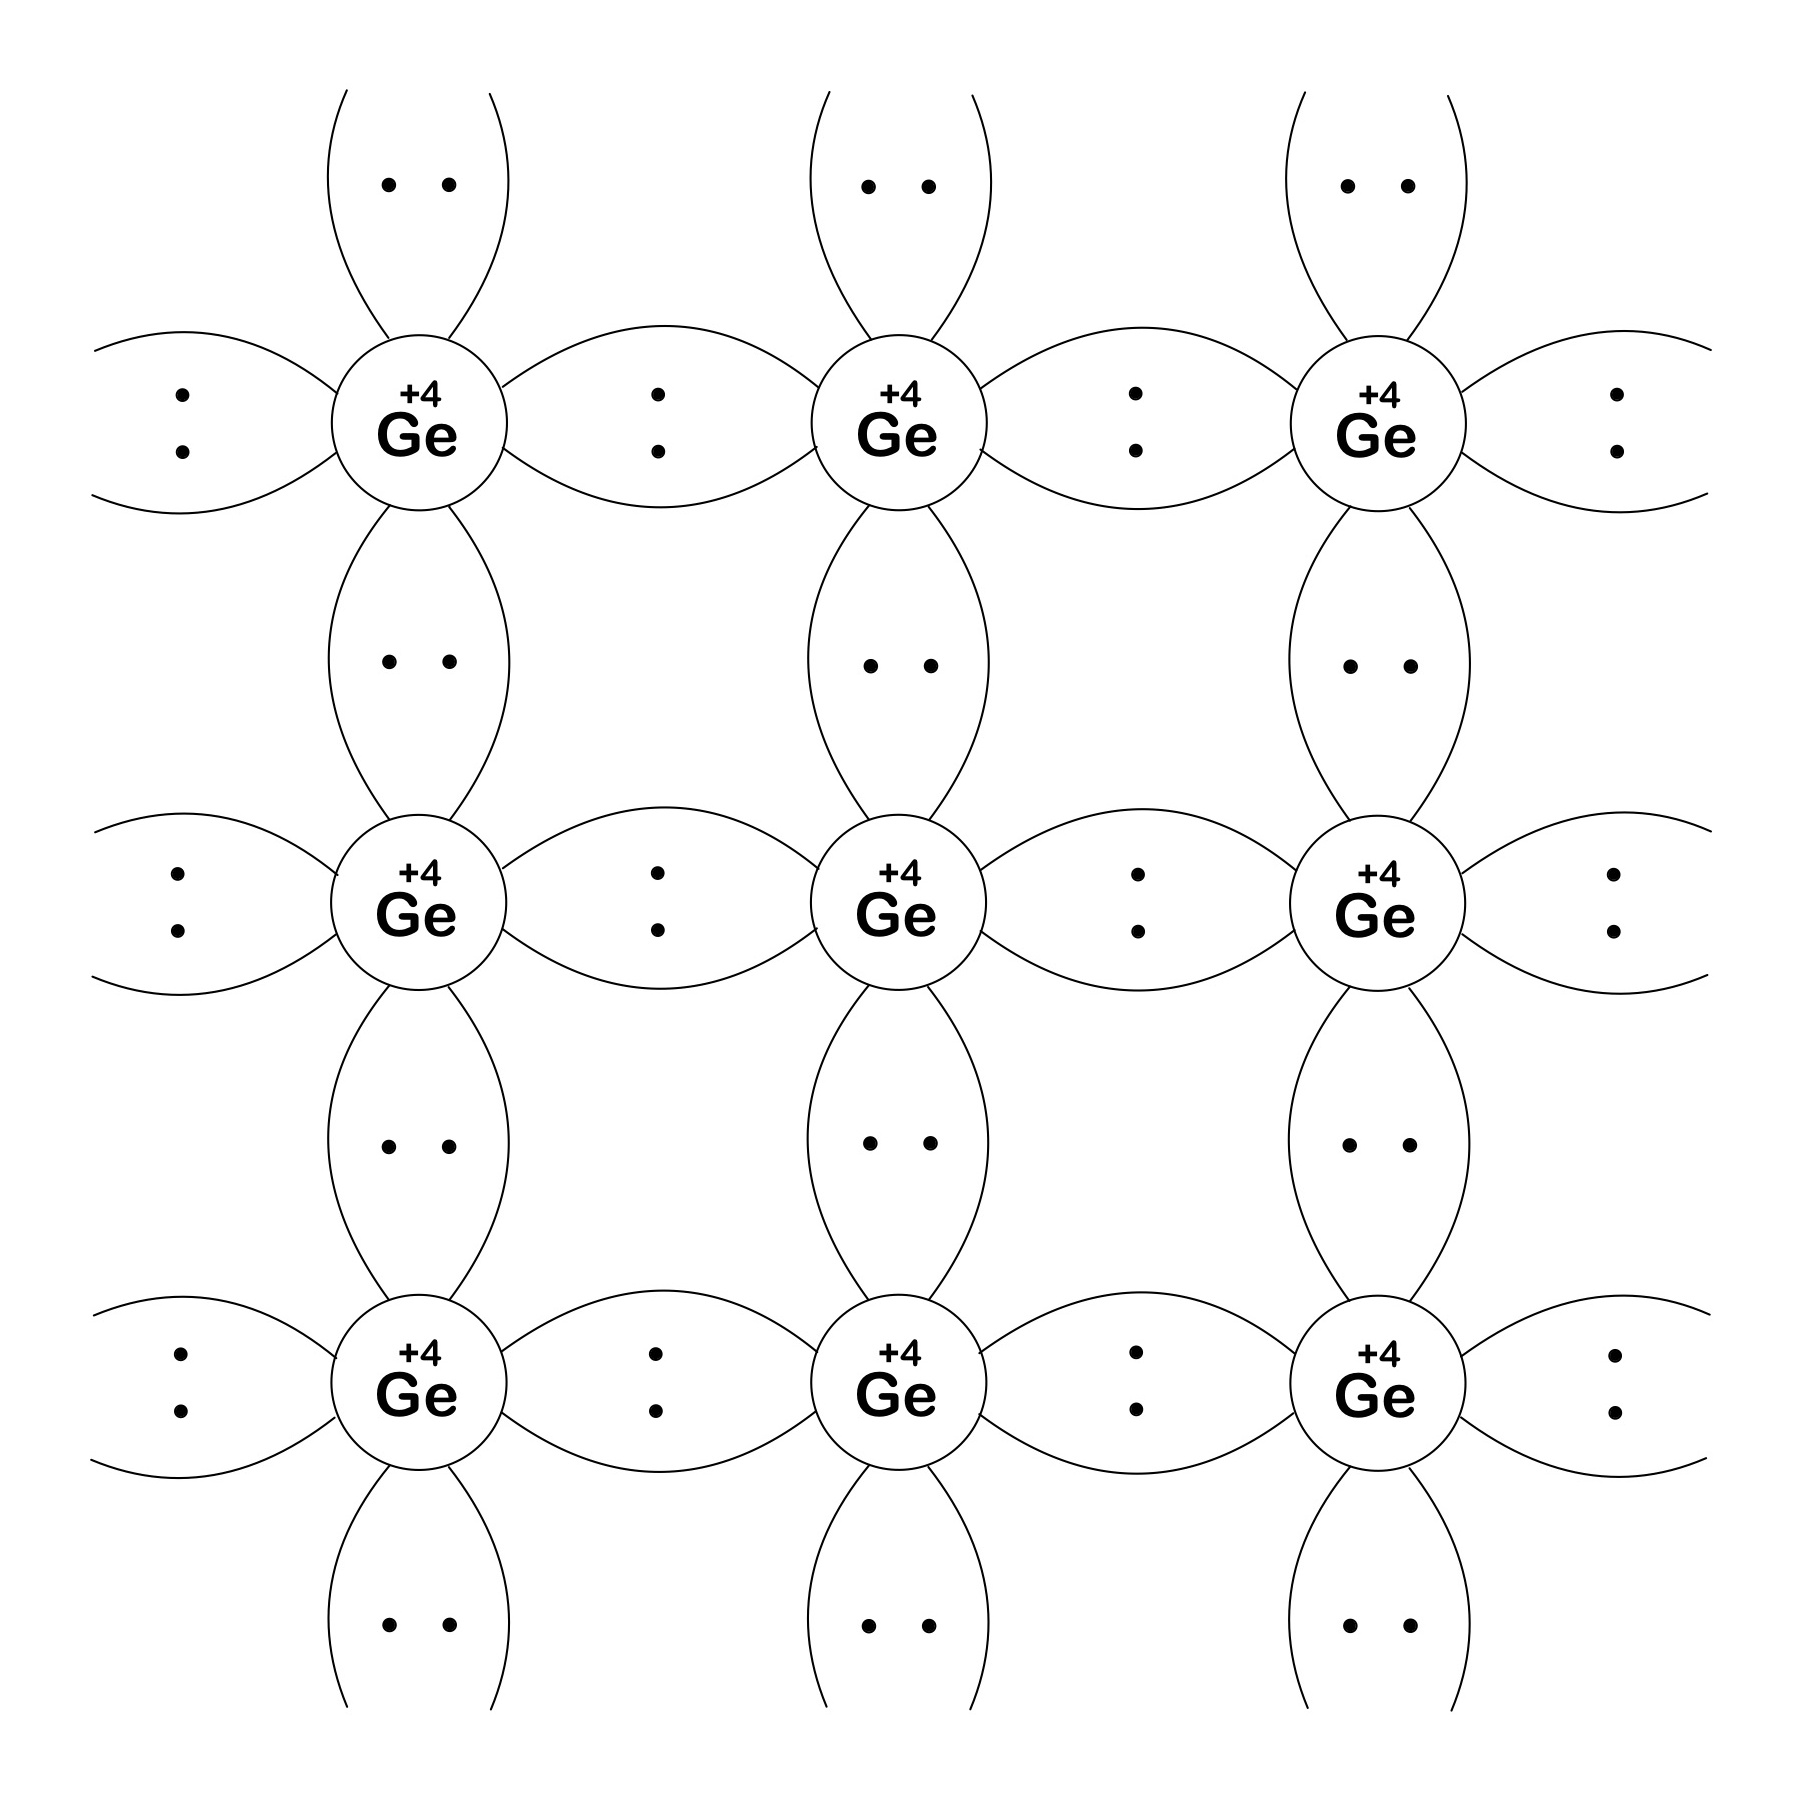
\includegraphics[width=0.333\textwidth]{figures/pureGermanium_square.jpg}\hfill
%     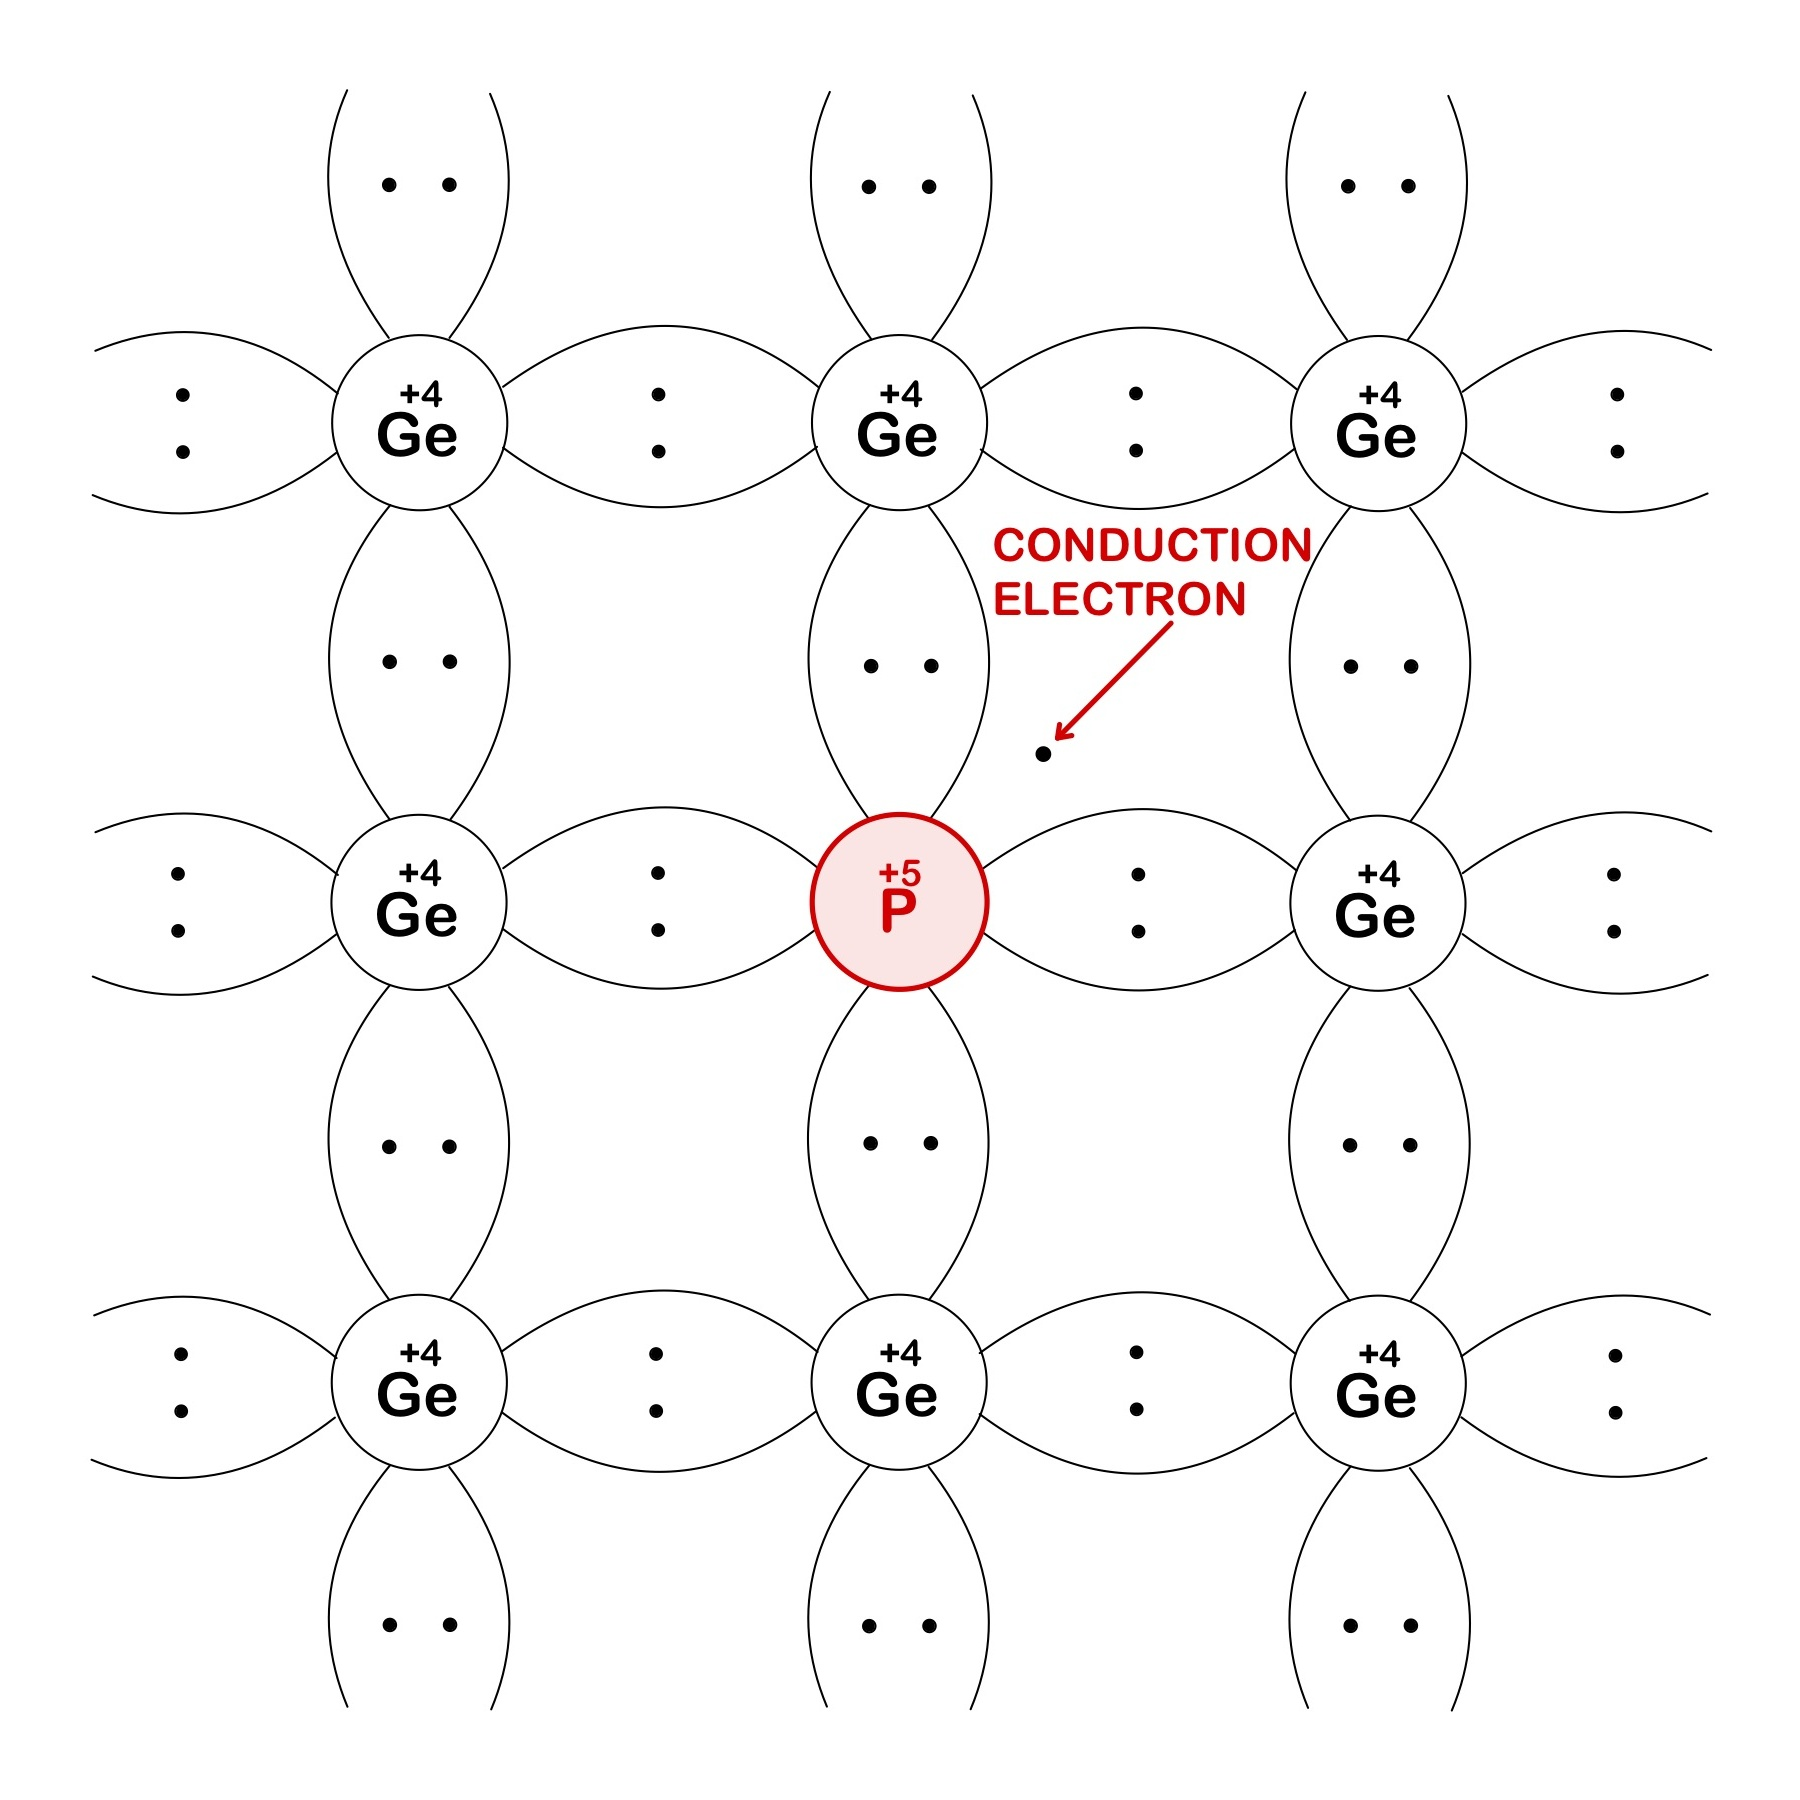
\includegraphics[width=0.333\textwidth]{figures/nDopedGermanium_square}\hfill
%     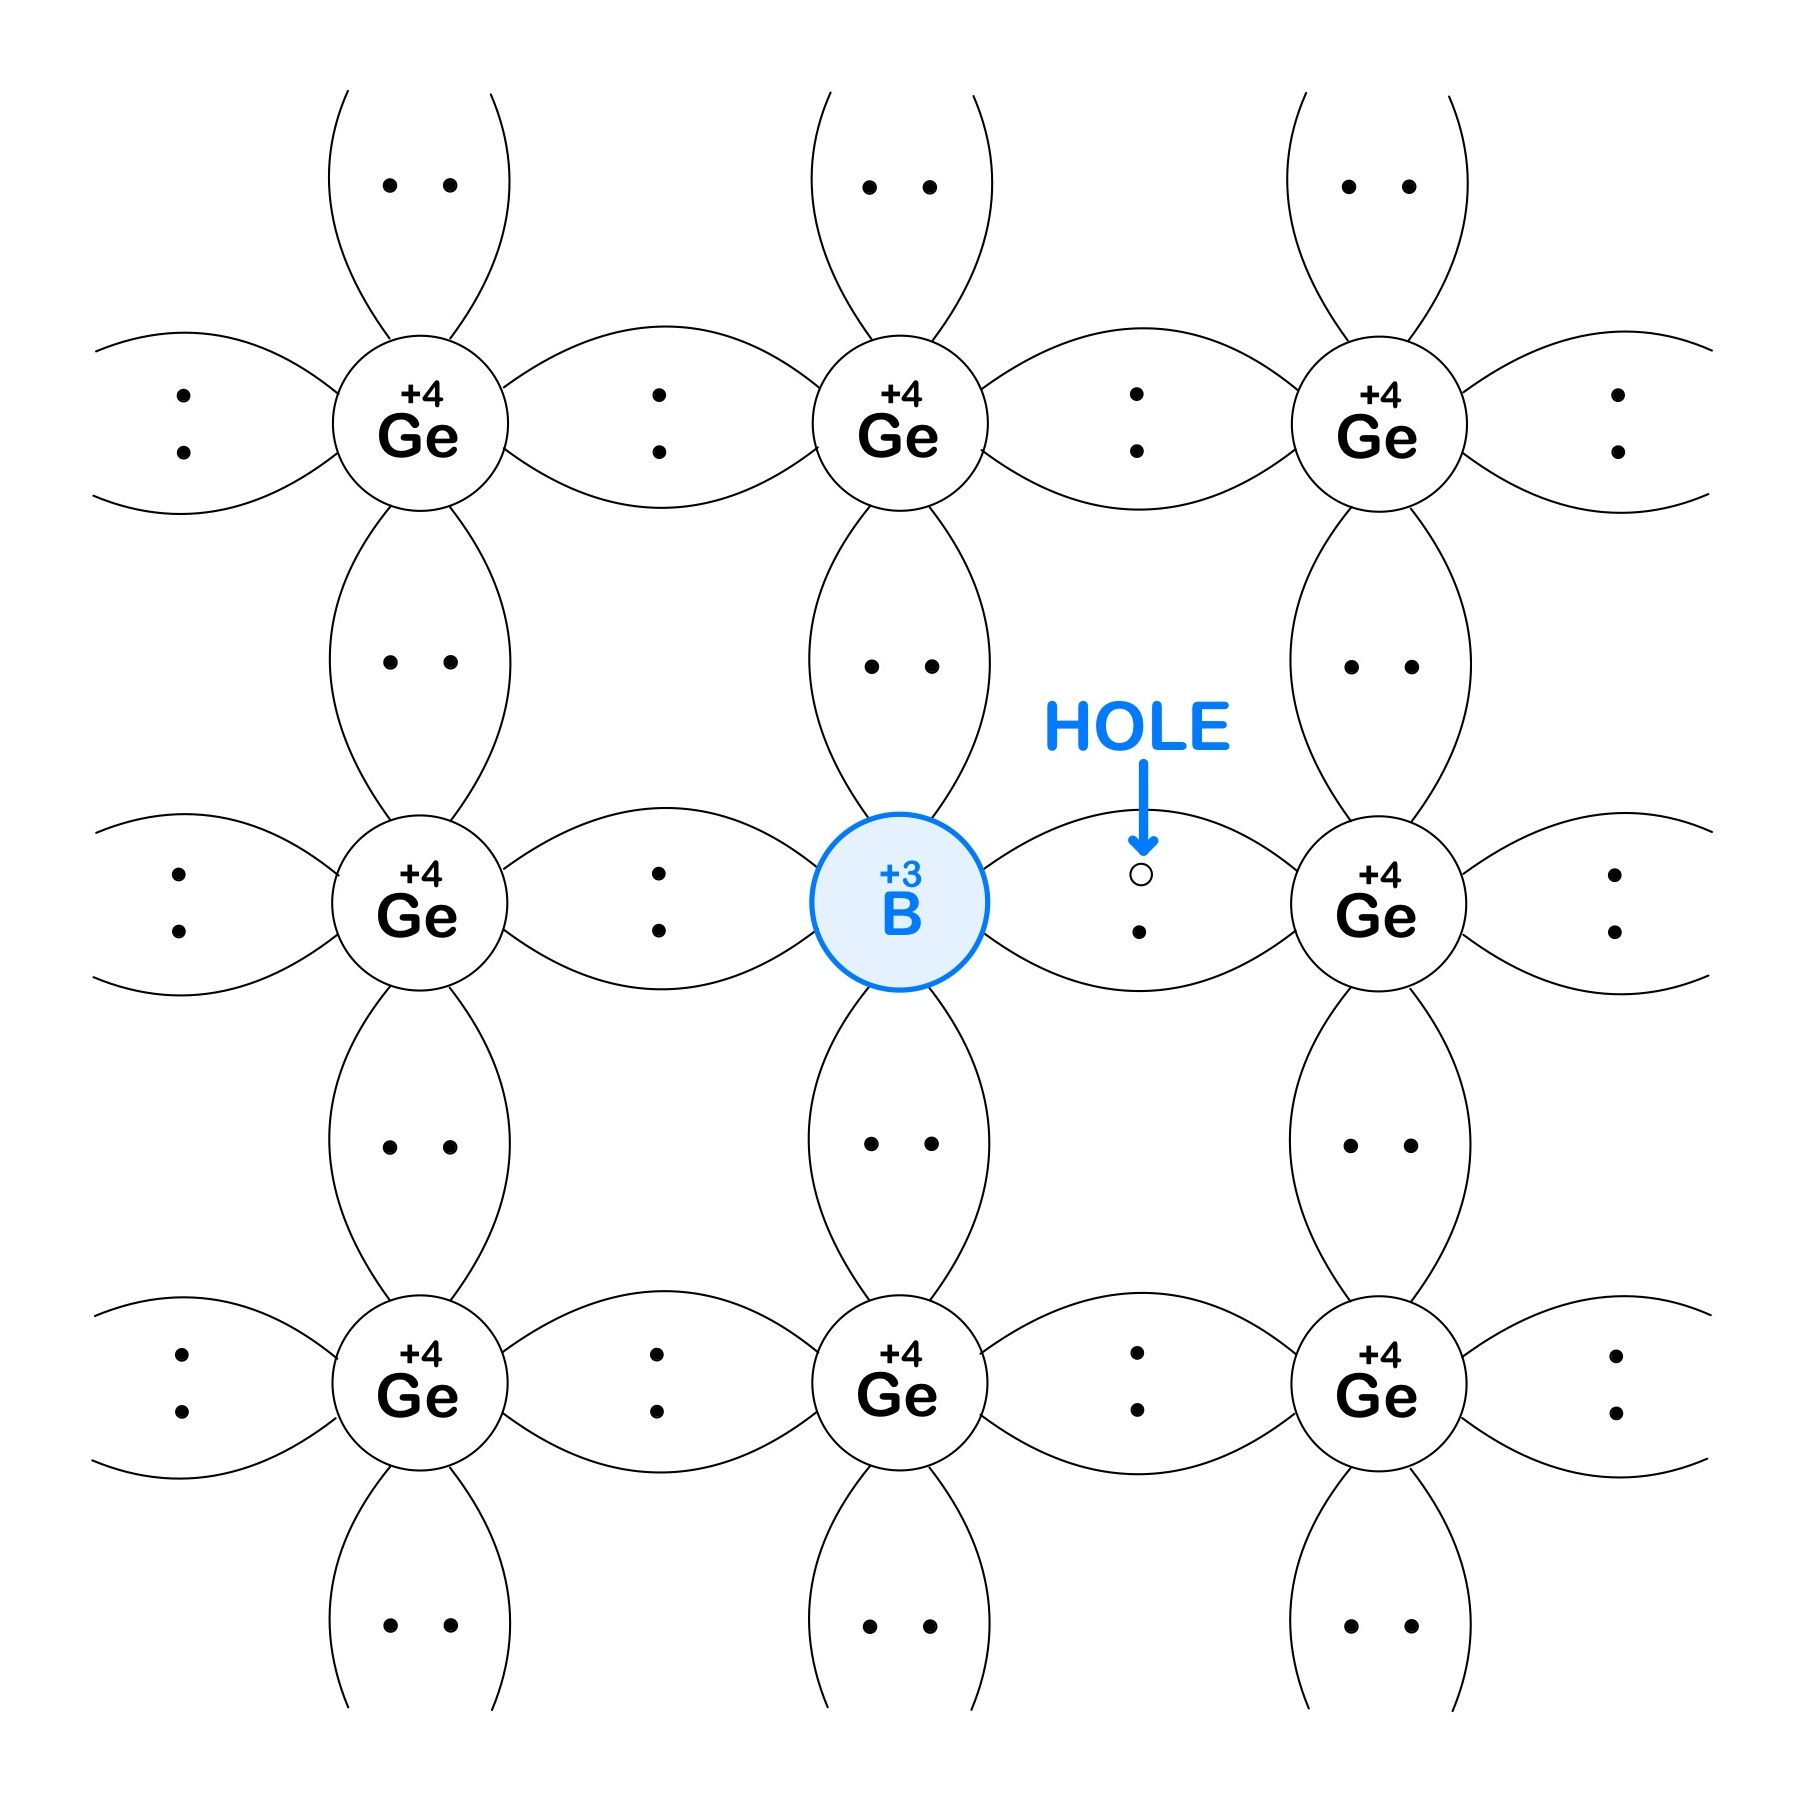
\includegraphics[width=0.333\textwidth]{figures/pDopedGermanium_square.jpg}
%     \caption{Germanium lattice configurations: on the left the pure Germanium crystal, in the center and on the right n-doped and p-doped Germanium respectively. Original drawing.}
%     \label{fig:intrisc-vs-extrinsic}
% \end{figure}

% \subsection{Germanium diodes in LEGEND-200}
% \begin{wrapfigure}{r}{0.3\textwidth}
%     \vspace{-1.2em}
%     \centering
%     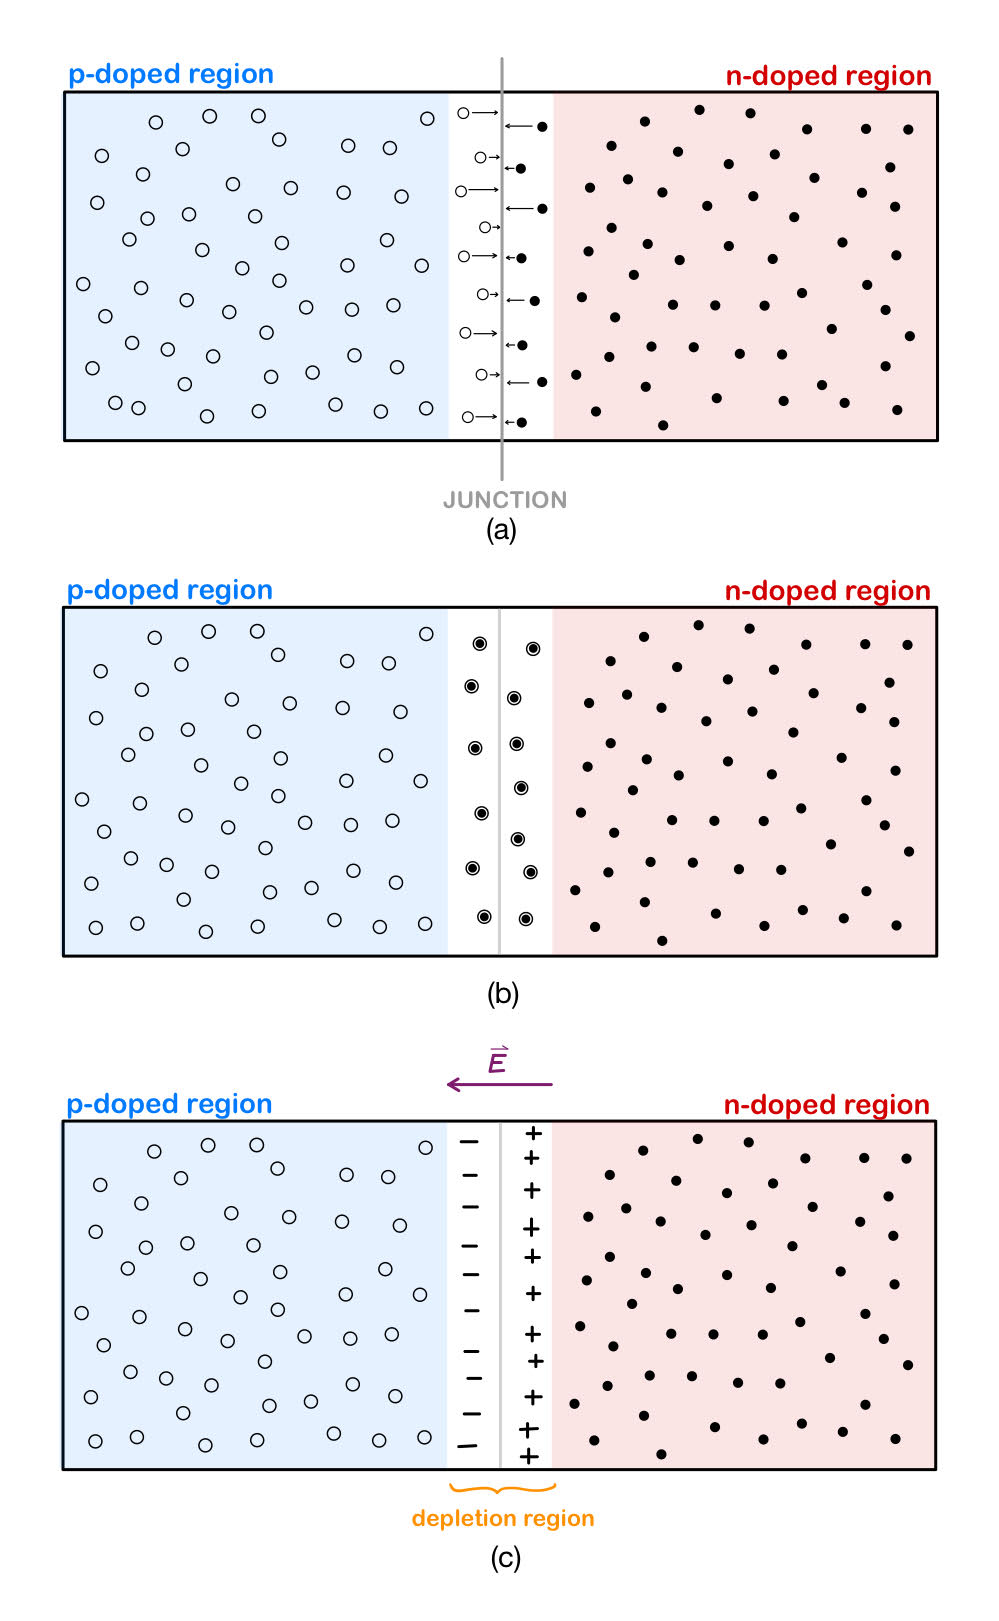
\includegraphics[width=\linewidth]{figures/diodi_introduzione1.jpg}
%     % \caption{Original drawing of junction creation (a), charge recombination (b) and depletion region formation (c)} %, bias voltage application (d) and full depletion (d).}
%     % \label{fig:diodi-intro}
% \end{wrapfigure}
When a p-type and an n-type semiconductor are joined within a single continuous crystal lattice, they form a fundamental interface known as a \textit{p-n junction}. Due to the steep concentration gradient at this boundary, majority charge carriers begin to diffuse across the junction: free electrons migrate from the n-side to the p-side, while holes diffuse in the opposite direction. As these mobile carriers cross the interface and recombine, they leave behind fixed, uncompensated ionized dopant atoms.
This process creates a localized volume depleted of mobile charge carriers, appropriately named the \textit{depletion region} (or space-charge region). The immobile ions within this region establish a built-in electric field that eventually opposes further carrier diffusion. This built-in electric field is further intensified when a bias voltage is applied across the p-n junction. At the same time, the depletion region extends deeper into the crystal, reaching its maximum extension when the applied voltage equals the so-called depletion voltage.
% \\
% \begin{figure}[H]
%     \centering
%     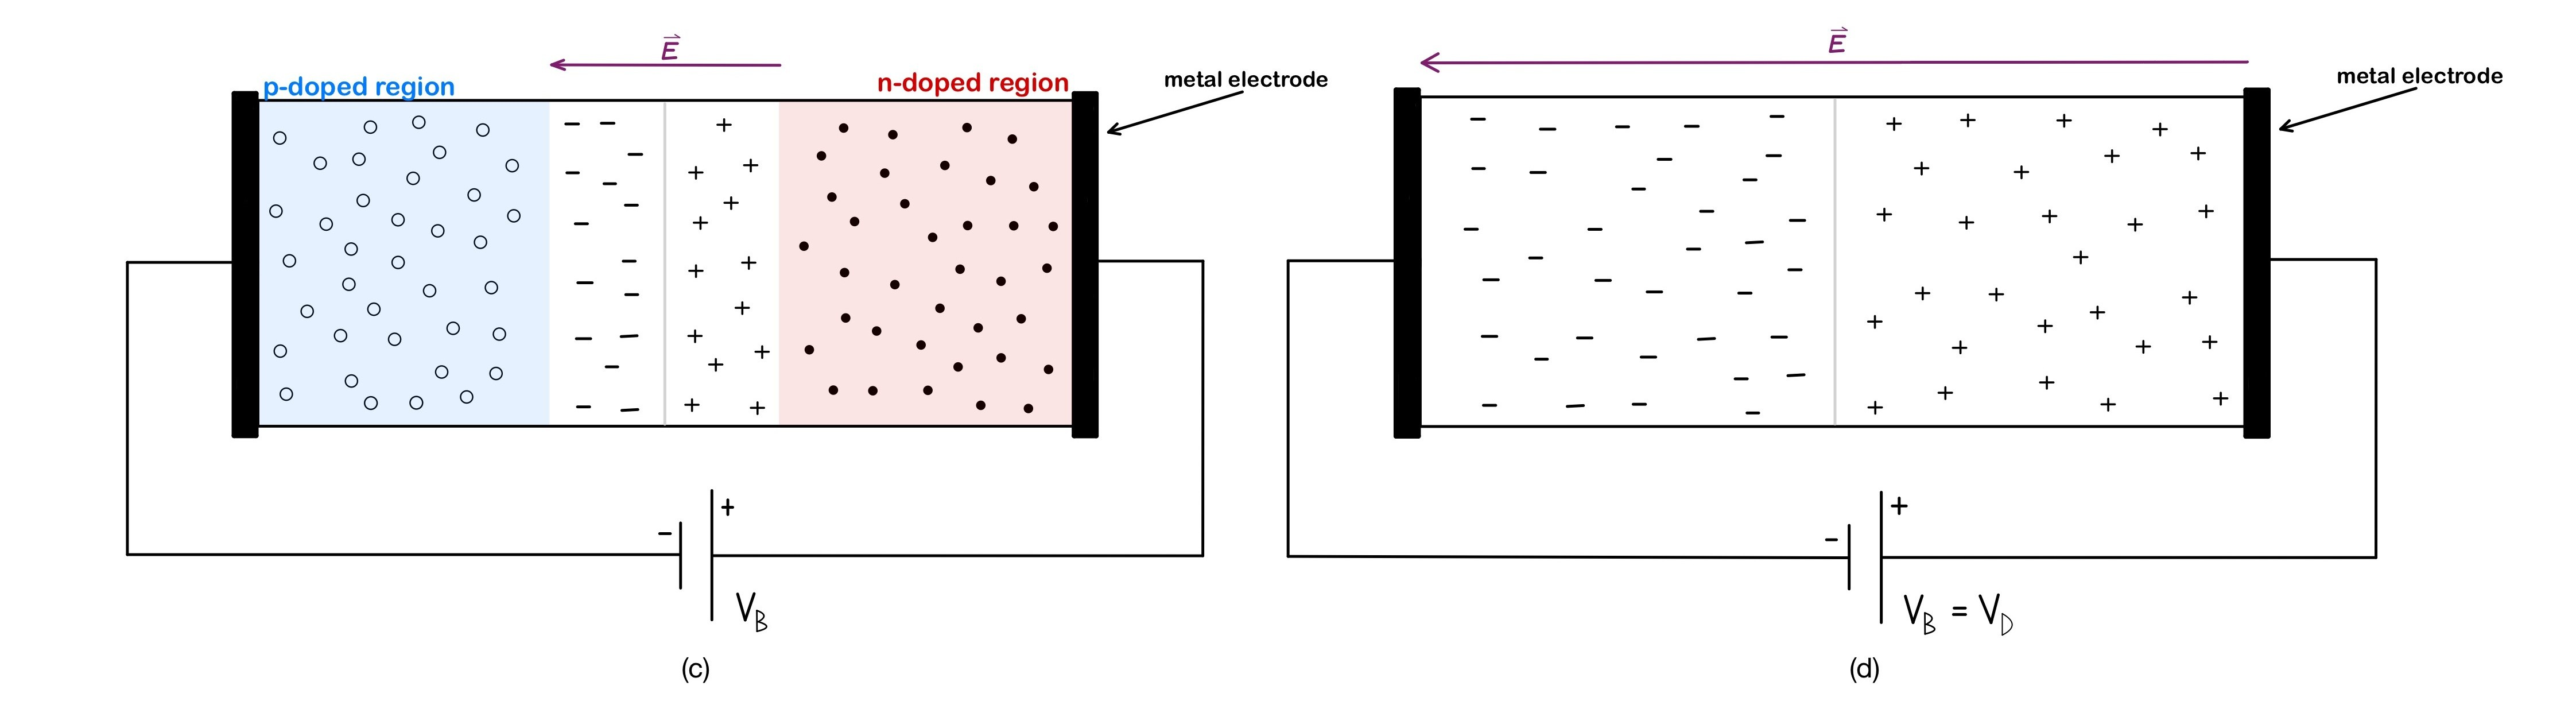
\includegraphics[width=\linewidth]{figures/diodi_introduzione2.jpg}
%     \caption{Original drawing of junction creation (a), charge recombination (b) and depletion region formation (c), bias voltage application (d) and full depletion (d).}
%     \label{fig:diodi-intro}
% \end{figure}

The p-n junction serves as the essential building block of modern semiconductor technology in its simplest two-terminal configuration within an electrical circuit; LEGEND Germanium detectors are exactly this type of semiconductor diode. Specifically, LEGEND diodes are built from a p-doped core where the p-n junction is formed with a highly doped n-type electrode, i.e. the \textit{n+} surface. The opposite part of the detector volume, on the contrary, is the so called \textit{p+}-doped contact. When a bias voltage is applied, a depletion region starts forming from the \textit{n+} part and reaches the \textit{p+} part when the voltage operation corresponds to the depletion voltage. 
% \begin{figure}[H]
%     \centering
%     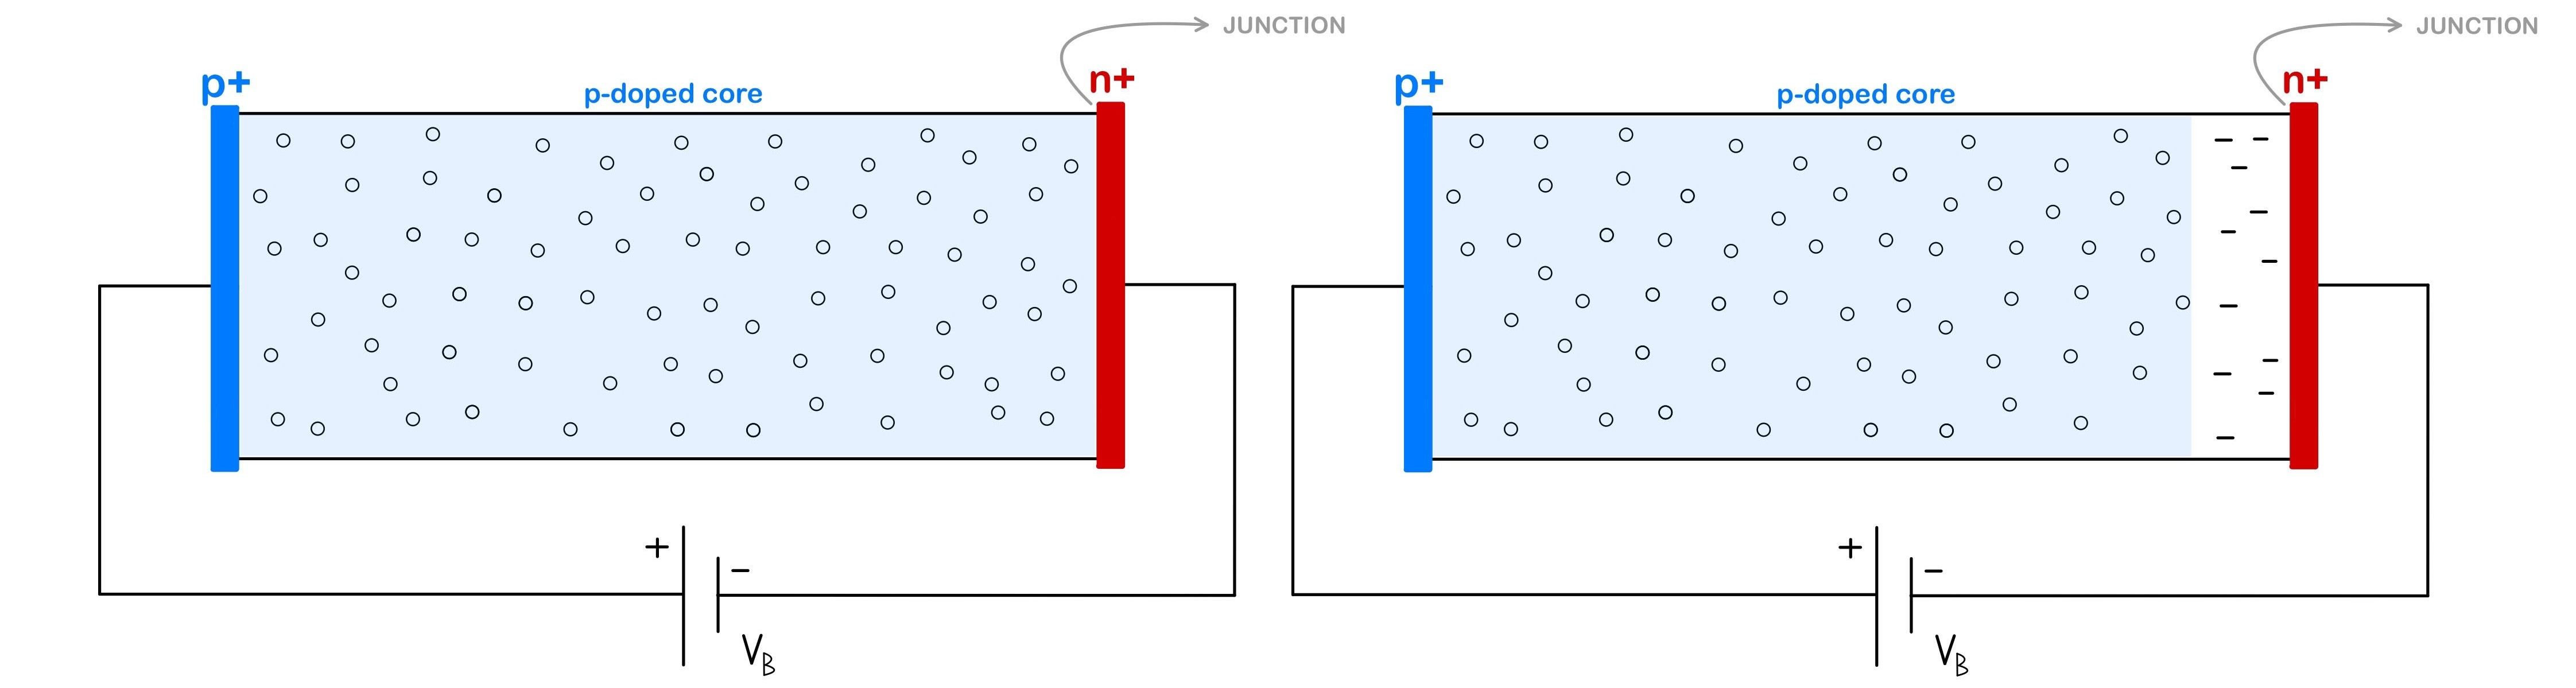
\includegraphics[width=0.8\textwidth]{figures/diodi_legend1.jpg}
% \end{figure}
% \begin{figure}[H]
%     \centering
%     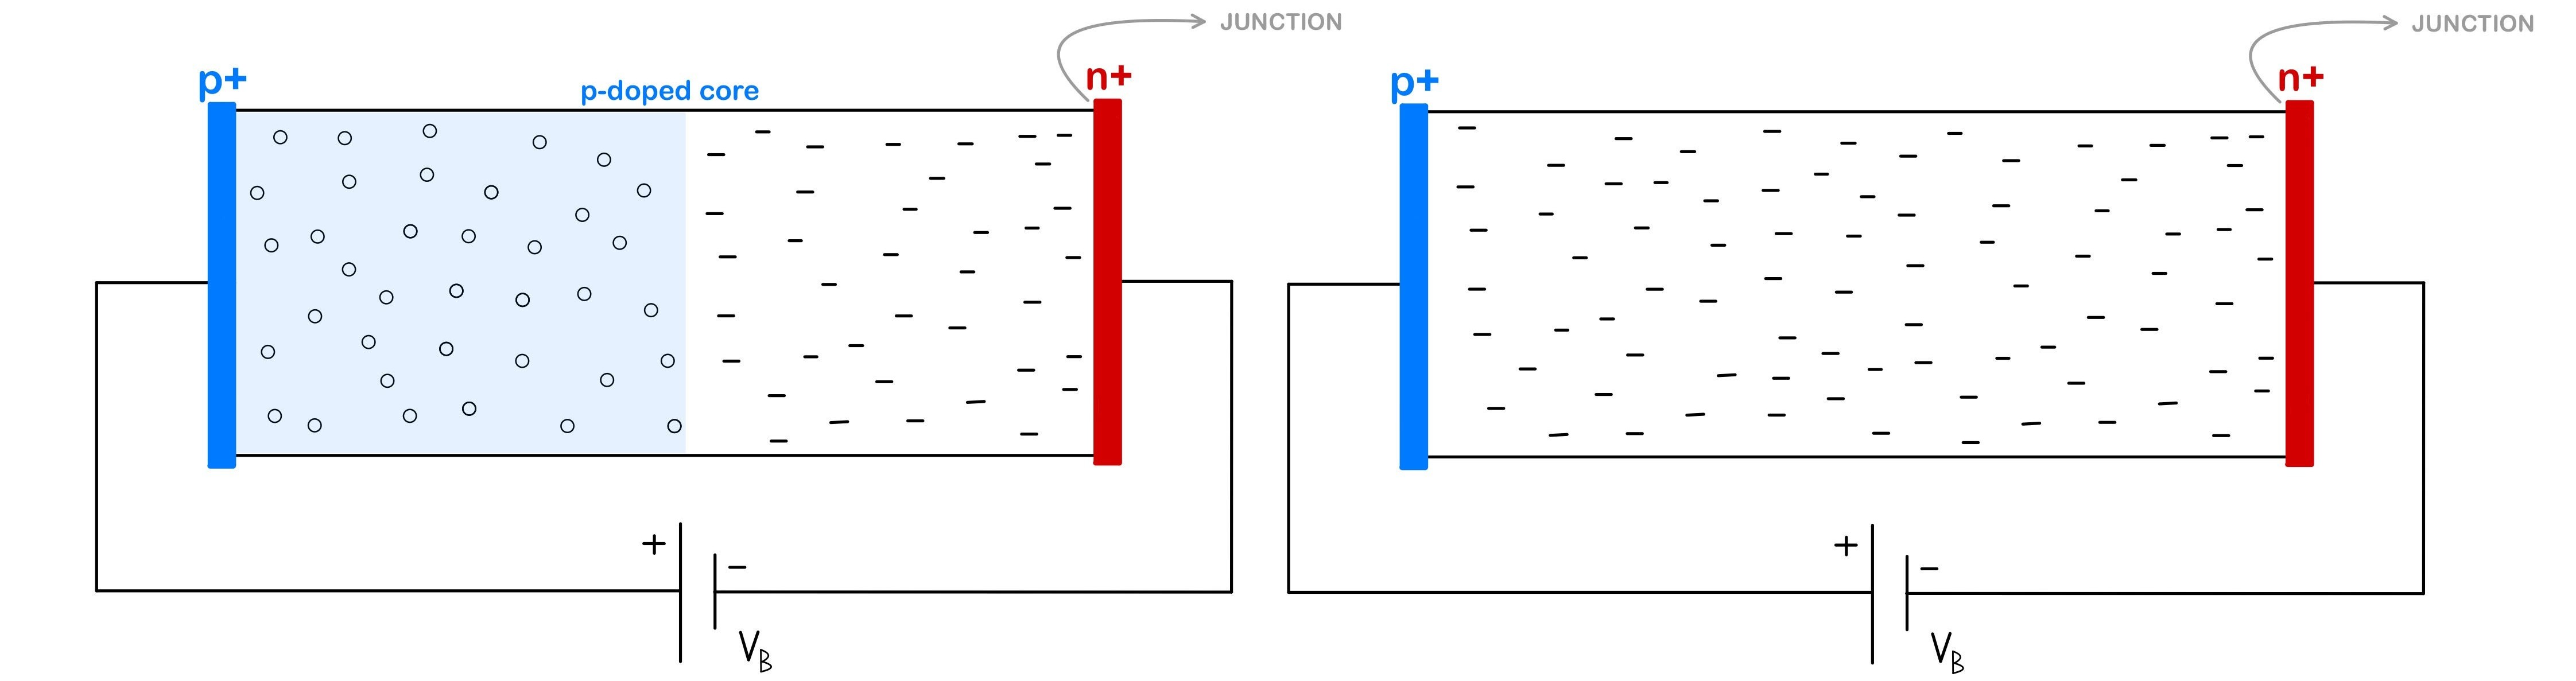
\includegraphics[width=0.8\textwidth]{figures/diodi_legend2.jpg}
%     \caption{Original drawing of the depletion voltage application for LEGEND diodes.}
%     \label{fig:diodes-legend}
% \end{figure}
Therefore Fig \ref{fig:detectors-types} can be developed highlighting the \textit{p+} part of the detector, as shown in Fig. \ref{fig:detectors-pINred}.
\begin{figure}[H]
    \centering
    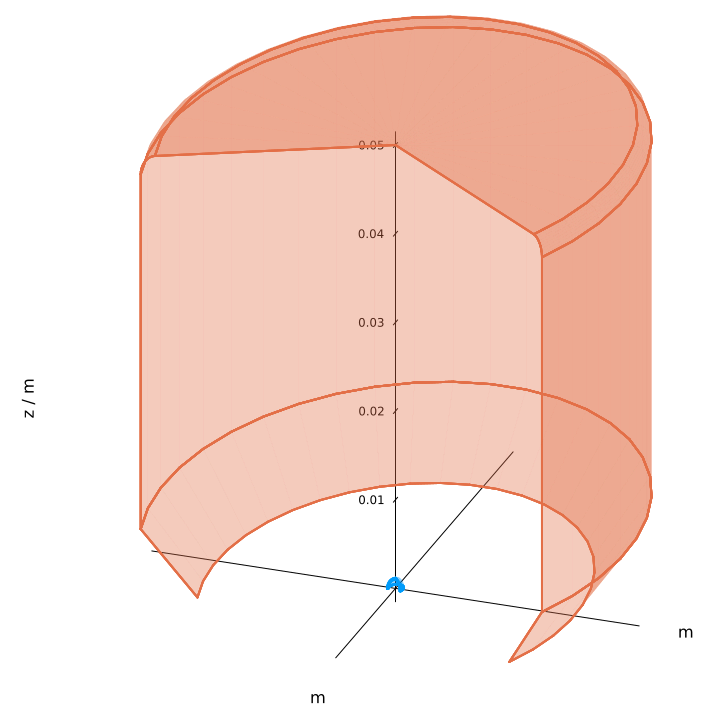
\includegraphics[width=0.25\textwidth]{figures/renderingDetectors/PPC_section_frontale.png}\hfill
    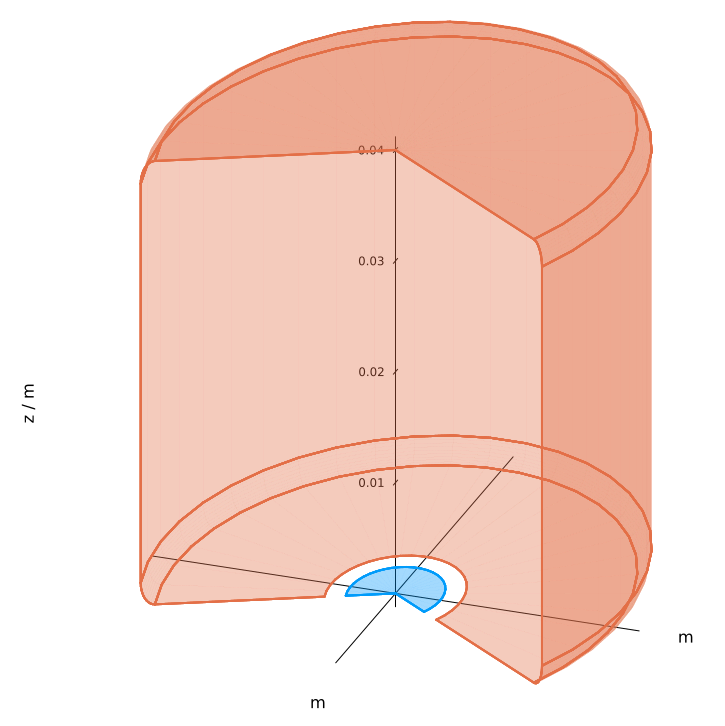
\includegraphics[width=0.25\textwidth]{figures/renderingDetectors/BeGe_section_frontale.png}\hfill
    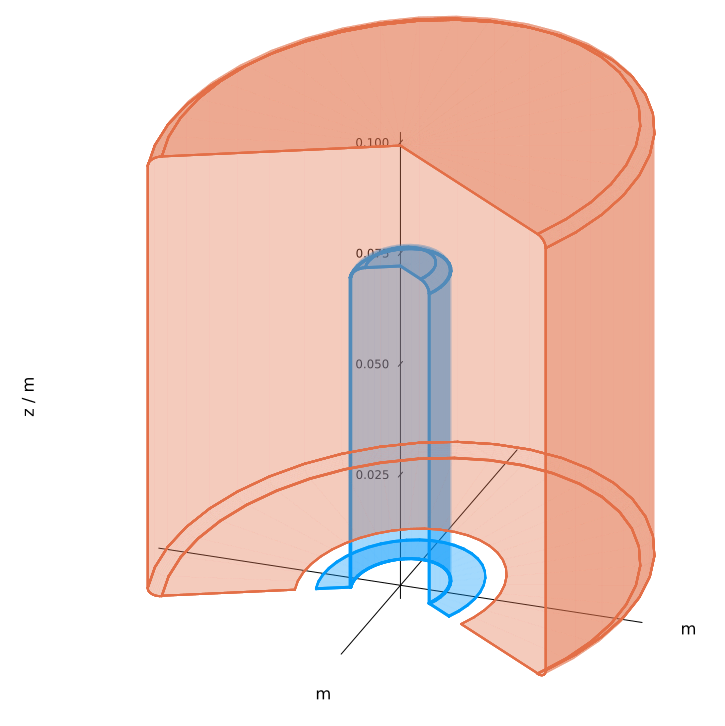
\includegraphics[width=0.25\textwidth]{figures/renderingDetectors/Coax_section_frontale.png}\hfill
    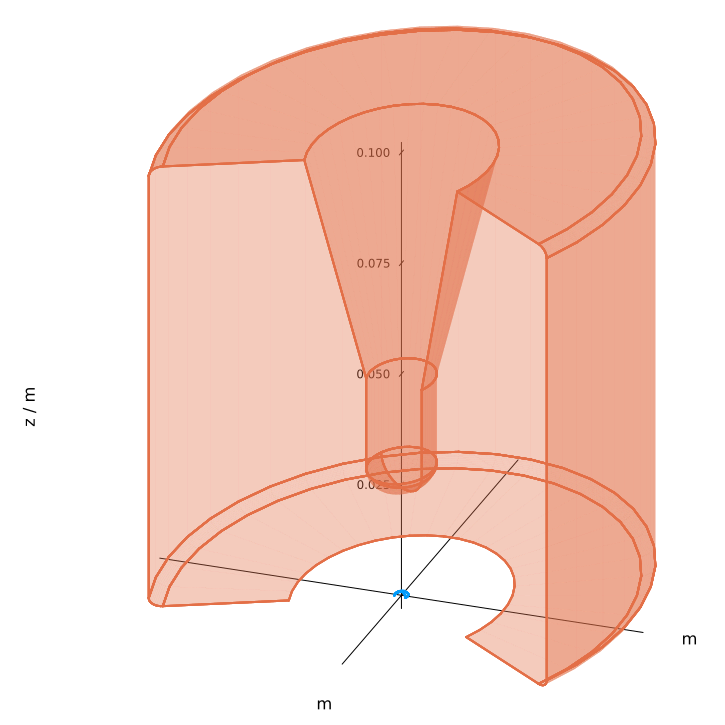
\includegraphics[width=0.25\textwidth]{figures/renderingDetectors/IC_section_frontale.png}
    \caption{Drawing of the different Germanium detectors employed in LEGEND. The \textit{p+} terminal IS highlighted in blue. From the left to the right: PPC, BEGe, Coax and IC detectors respectively. Rendering scripts are by D. Hervas.}
    \label{fig:detectors-pINred}
\end{figure} 
When the entire detector volume becomes active and sensitive to ionizing radiation, if an incoming particle or gamma ray deposits energy within this volume, electron-hole pairs are generated in proportion to the deposited energy (in germanium, creating a single \ac{eh} pair requires 2.96 eV). Driven by the electric field, holes drift toward the \textit{p+} contact and electrons toward the \textit{n+} contact, inducing a measurable signal.

\begin{wrapfigure}{r}{0.47\textwidth}
    \centering
    \begin{tikzpicture}
        % 1. Inserisce il PDF originale vettoriale
        \node[anchor=south west, inner sep=0] (plot) at (0,0) {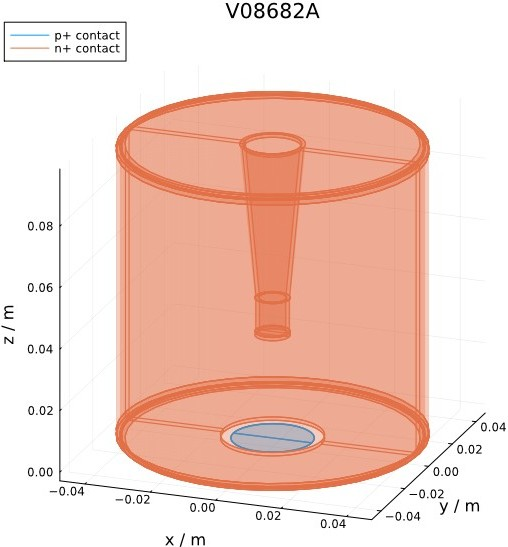
\includegraphics[width=\linewidth]{figures/ramo-shockley/geometry_V08682A-def.jpg}};
        
        % 2. Sovrappone il logo in alto a destra
        % (Regola width=1.5cm e gli shift per adattarli alla dimensione del wrapfigure)
        \node[anchor=north east, inner sep=0, xshift=-5pt, yshift=0pt] at (plot.north east) {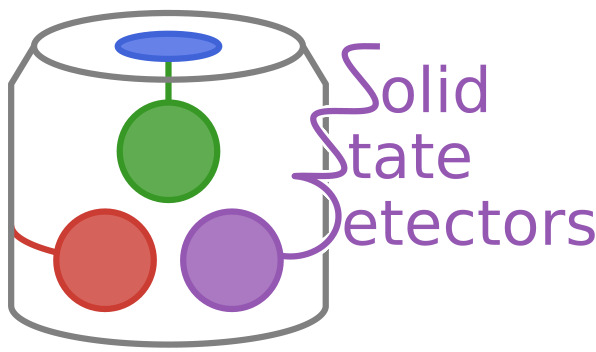
\includegraphics[width=2cm]{figures/ramo-shockley/logo_SSD.jpg}};
    \end{tikzpicture}
    \captionsetup{font=small}
    \caption{Geometry of the detector V08682A. Own elaboration based on LEGEND detector specifications using Julia-based SolidStateDetectors software \cite{SSD-jl}.}
    \label{fig:V08682A}
\end{wrapfigure}
While the LEGEND-200 experiment employs all the detector geometries of Fig. \ref{fig:detectors-types}, the work presented in this thesis focuses exclusively on a single Inverted Coaxial (IC) detector, labelled V08682A. Its rendering is shown in Fig. \ref{fig:V08682A}. Said detector was manufactured by MIRION which ensures an ${}^{76}$Ge enrichment fraction of (90 $\pm$ 1)\%. The mass is $m = 3340~\text{g}$, and it is $95.7~\text{mm}$ high. The overall radius is $r = 45~\text{mm}$. The \textit{p+} contact is highlighted in blue in the picture and its radius is $r_{\mathit{p+}} = 12~\text{mm}$; the \textit{n+} electrode (the HV one) is given by all the surface of the detector, depicted in orange. Between the two, on the bottom face of the detector, lies the passivated groove: a narrow ring-like surface that is 2 mm deep and has an inner radius of 12 mm and an outer one of 15 mm. Since SolidStateDetectors software only colours biased electrodes, this groove appears as the uncolored part between the orange \textit{n+} and the blue \textit{p+}. The detector operates at a bias voltage of V$ = 3500~\text{V}$, recommended by the LEGEND-200 site characterization with an adequate safety margin above the depletion voltage of~$3000~\text{V}$ to ensure the operation of the detector in full depletion condition which translates into maximal active volume.
Restricting the scope of the work solely to this detector is a methodological choice: the algorithm developed as the primary goal of this thesis requires robust initial validation on a specific, well-characterised detector. Its generalization to the remaining detectors is left as a future prospect, outside the boundaries of this work. 
% that will be worth only if the first trial returns significantly good results. 
Hence, all of the following physics principles, data analyses and algorithm implementations discussed herein are tailored specifically to the IC V08682A detector.

\subsubsection{Signal formation in Germanium detectors}
\paragraph{The Shockley-Ramo theorem}
Consider, for instance, an incident $\gamma$-ray that interacts with the semiconductor and generates a large number of \ac{eh} pairs proportional to the deposited energy \footnote{Similarly, in the search for $0\nu\beta\beta$ decay, the kinetic energy of the emitted electrons acts as the ionizing source, generating a signal proportional to the decay energy.}. The movement of these electrons and holes, for a total moving charge \textit{q}, due to the electric field within the device, causes a variation of the induced charge \textit{Q} on an electrode. The change of \textit{Q} is converted to a voltage pulse using a charge sensing amplifier and the amplitude of the output voltage signal ideally is proportional to the deposited energy.

The time-dependent output signal of a charge sensing device can be predicted if the induced charge \textit{Q} on the readout electrode can be calculated as a function of instantaneous position of the moving charge \text{q} within the device. The Shockley-Ramo theorem (\cite{Shockley}, \cite{Ramo}), originally developed for vacuum tubes, can be applied also in the case of stationary space charges of the abovementioned \ac{hpge}. 

From this theorem we know that the charge \textit{Q} and current \textit{i} on a selected electrode induced by a moving point charge \textit{q} are given by
\begin{equation}
    \label{eq:carica-corrente-SR}
    \begin{gathered}
        Q = - q \, \varphi_\text{w} (\mathbf{x}) \\~\\
        i = \frac{\text{d}Q}{\text{d}t} = -q \, \frac{\text{d}\varphi_\text{w} (\mathbf{x})}{\text{d}t} = -q \left( \nabla \varphi_\text{w}(\mathbf{x}) \cdot \frac{\text{d}\mathbf{x}}{\text{d}t} \right) = q \, \mathbf{v} \cdot \mathbf{E}_\text{w}(\mathbf{x})
    \end{gathered}
\end{equation}

where $\mathbf{v}$ is the instantaneous velocity of the charge \textit{q}. The terms $\varphi_\text{w}(\mathbf{x})$ and $\mathbf{E}_\text{w}(\mathbf{x})$ are, respectively, the \textit{weighting potential} and the \textit{weighting field} evaluated at the instantaneous position $\mathbf{x}$ of the charge. They are defined as the potential and the electric field that would exist in the device if the selected electrode were set to a unit potential, with all other electrodes grounded (set to zero potential) and all space charges removed. \cite{GeDetectors}


\paragraph{IC weighting field}
% As already sentenced above in Sec. \ref{subsec:Ge-detector-basics}, the work focuses on V08682A IC detector, therefore what follows is the analysis of the weighting field in this specific detector geometry. 
IC detectors in LEGEND feature a well on the opposite side of the p-contact to increase the electric field in the upper part of the detectors and make it possible to drift the charge. MIRION IC detectors, as the one considered in this work, exhibits a straight/tapered well, visible in Fig. \ref{fig:V08682A}. \cite{lnote_21003}

The structure of an IC detector creates a region surrounding the \textit{p+} electrode with a very high weighting field, as is visible in Fig. \ref{fig:weighting}. This means that, when an \ac{eh} pair is produced, the pulse shape of the signal is almost entirely determined by the holes drifting towards the \textit{p+} contact, rather than the electron-induced one which can be considered negligible. In principle, the shape of the current signal varies depending on where the physical process happen with respect to the readout electrode; however, seeing that far away from the \textit{p+} electrode  the field is very low, which means that the current signal that is proportional to the field (see Eq. \ref{eq:carica-corrente-SR}) is negligible, we can assume that wherever the physical process happens, the real signal only starts when the hole is sufficiently near to the point contact. Nonetheless, if the event happens very close to the \textit{p+} electrode, holes rapidly drift to it. On top of that electrons are generated within the high-weighting-field region and induce a sizeable current while drifting away from it, before entering the region where $\text{E}_\text{w}$ is negligible. \cite{dissertationComellato}

\begin{figure}[H]
    \centering
    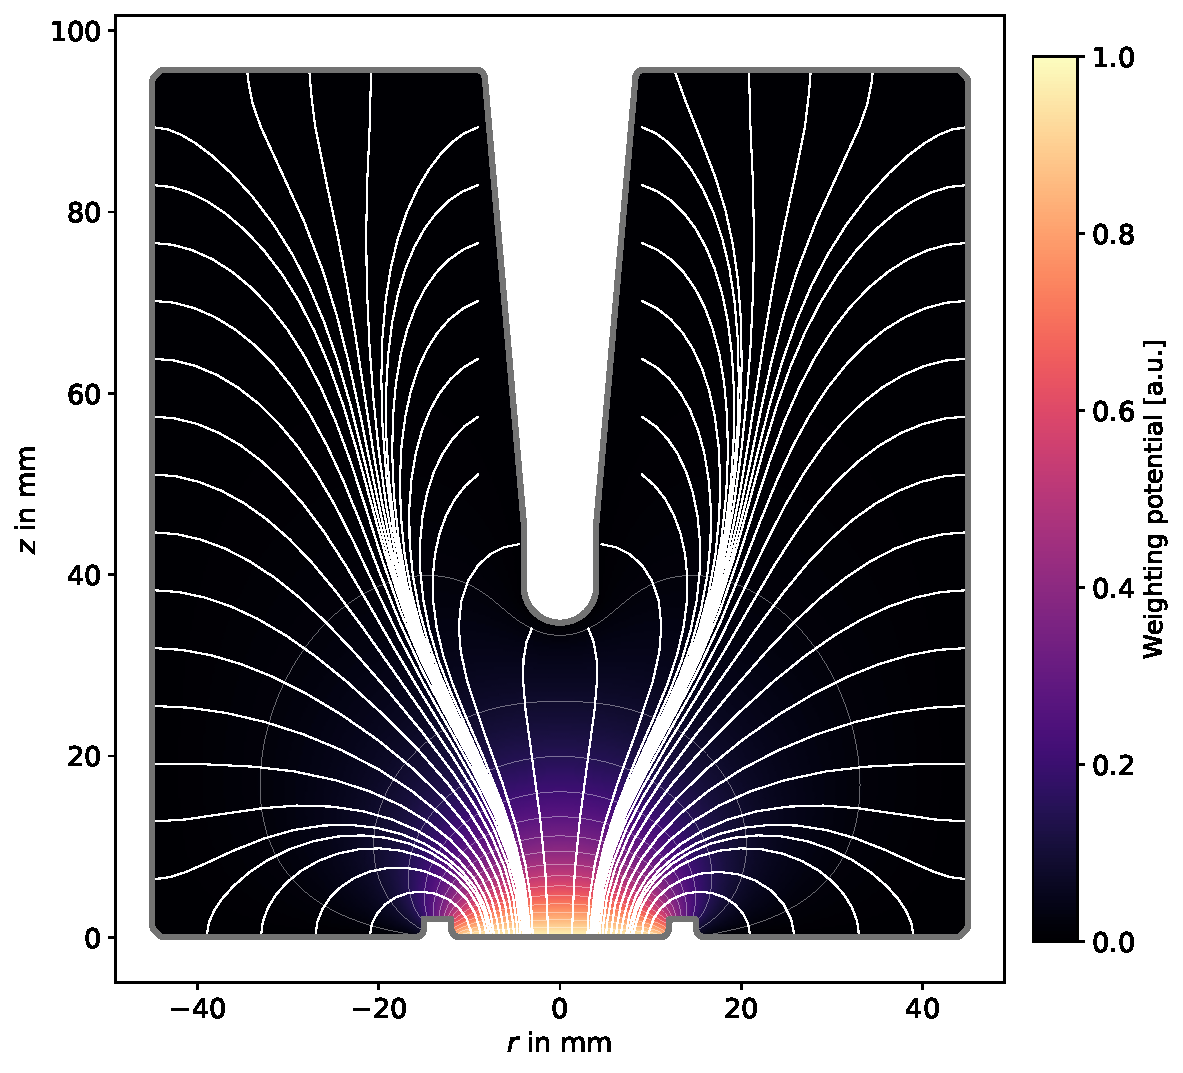
\includegraphics[width=0.48\textwidth]{figures/ramo-shockley/V08682A_weighting_potential.pdf}\hfill
    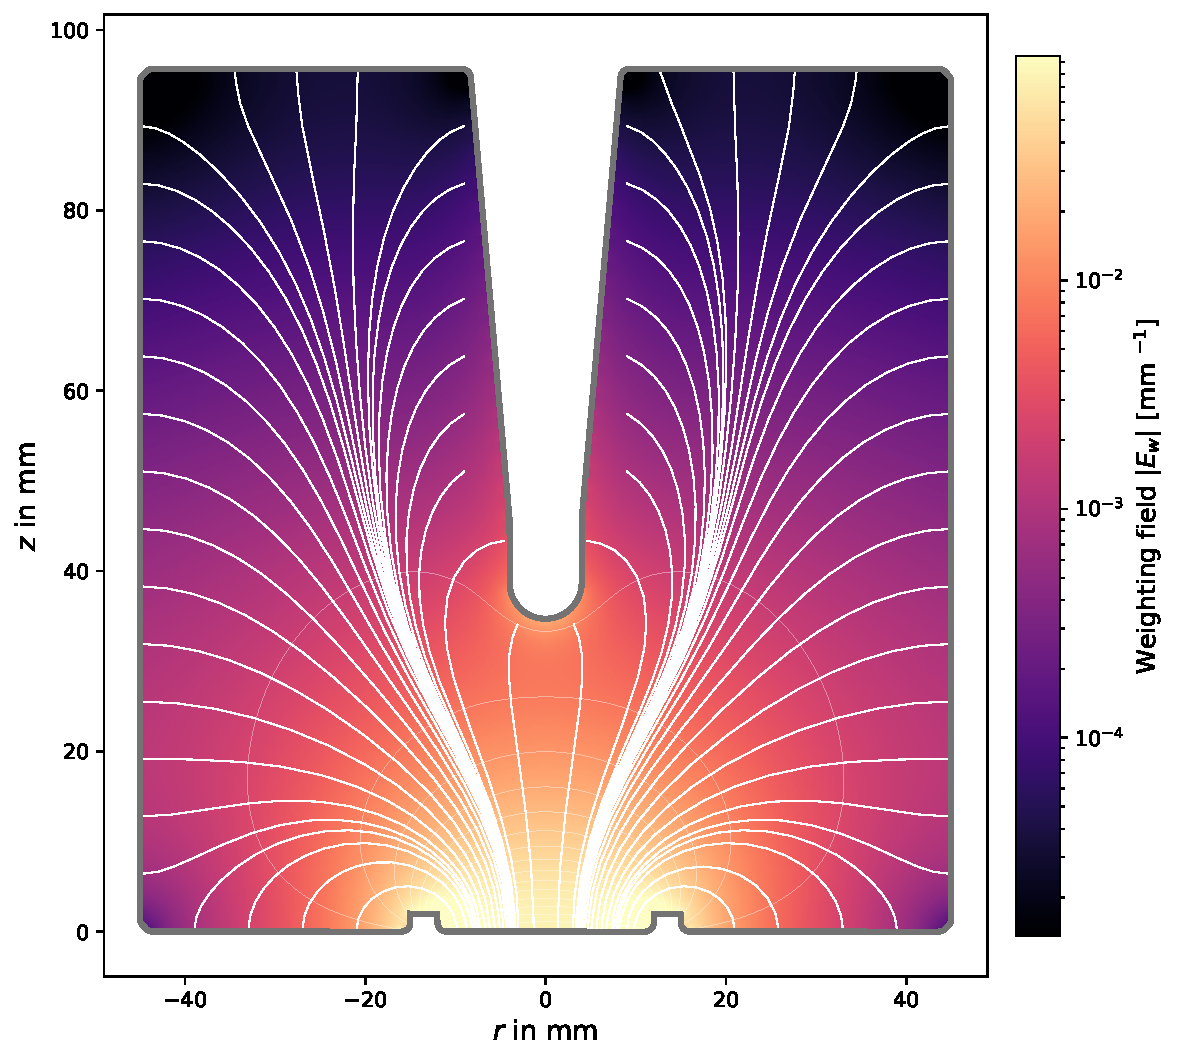
\includegraphics[width=0.48\textwidth]{figures/ramo-shockley/V08682A_weighting_field.pdf}
    \caption{Weighting potential (left) and weighting field (right) in the V08682A IC detector. Own elaboration based on LEGEND Metadata.}
    \label{fig:weighting}
\end{figure}

\subsubsection{Events topology}
\label{subsubsec:topology}
The shape of the recorded signals depends on how many energy depositions are associated with the very same initial physical process and on how they are distributed in space and in time within the detector volume. This dependence makes it possible to discriminate between different event topologies, which in turn correspond to different underlying physical processes.

When a physical event produces only one energy deposition, charge carriers are generated all at once in a single localised point in the detector and they drift along the same trajectory. The resulting signal registered by the detector has a simple, prompt shape. Such an event is referred to as a \ac{SSE}.
Conversely when the same initial particle interacts several times at different positions inside the detector ---as in multiple Compton scattering---, the charge carriers are created at different locations in space and at different moment in time. All of these individual contributions superimpose with one another and produce a current signal with a more complex and temporally extended structure. Said events are referred to as \ac{MSE}.
This distinction is precisely what makes pulse shape analysis a powerful background rejection method. In a neutrinoless double beta decay (0$\nu\beta\beta$), the two resulting electrons share the full Q$_{\beta\beta}$; at 1 MeV they have a range of the order of 1 mm in Germanium and thus they are rapidly absorbed giving rise to a \ac{SSE}-like signal. 
On the other hand, background processes with similar energies arise mainly from $\gamma$ interactions undergoing several Compton scattering before being totally absorbed and thus exhibits a \ac{MSE} topology. Hence, identifying \ac{SSE} behaviour with respect to \ac{MSE} means selecting signal-like events and rejecting \ac{MSE} ones which constitute an important part of the LEGEND background.

On top of that, another distinction is critical when it comes to events topology. Physical processes can occur both in the bulk of the detector and near the surface of it: these events are moslty $\alpha$ and $\beta$ emissions. The $n^+$ electrode is covered by a lithium-diffused layer (about $1$~mm for the detector considered here) which alpha particles cannot penetrate. On the other hand beta particles entering through it release their energy in a region of reduced electric field and produce characteristically slow pulses~\cite{L1000-design}. The opposite situation occurs at the $p^+$ contact and on the passivated surface of the groove, which separates the two electrodes: being only a fraction of a micrometer thick, they are fully exposed to both alpha and beta particles. To look into it further we need to analyse the physics in the groove region where the electric field\footnote{This is the physical electric field not to be confused with the Shockley-Ramo weighting field.} that drives charge drift runs parallel to the groove. However a perpendicular component arises from the fact that the groove is electrically floating and highly resistive thus can accumualte charge. This means that $\alpha$ and $\beta$ particles may generate a very slow readable signal characterised by the so-called \ac{DCR}. While alfas are totally affected by this process because of their very small range, betas that penetrate considerably more are only partially affected by it. Relevant emitters in this context are the $\beta$ decay of $^{42}$K in the surrounding liquid argon and the $\alpha$ decay of $^{210}$Po from the $^{222}$Rn progeny, both already introduced in Sec.~\ref{sec:background}: neither of these deposits energy exactly at $Q_{\beta\beta}$, but both of them can mimic a signal-like event once the observed energy is degraded. 

Classifying events according to the shape of their signal is the basis of \ac{PSD}, a powerful tool for signal-background discrimination that is the main focus of this thesis and will be detailed and developed in depth in Sec.~\ref{sec:traditionalPSD}. In particular, 0$\nu\beta\beta$ events are to be searched as bulk \ac{SSE} events in the correct energy region of interest.

\subsection{Data acquisition and processing}
\subsubsection{Readout electronics}
The \ac{DAQ} system for LEGEND-200 consists of FlashCam digitisers and an \ac{ORCA} \ac{DAQ} software. The \ac{DAQ} system employs a \ac{FADC} based on the FlashCam readout system, which digitises the detector signals with 16-bit precision at a 62.5 MHz sampling rate. An event is defined by the digitised signal crossing a threshold, set to an energy equivalent to approximately 20 keV. Each resulting trace consists of 8192 samples (131 $\mu$s), including both the pulse and a pretrigger baseline interval. \cite{LEGEND:GeDet} 

\begin{wrapfigure}{r}{0.5\textwidth}
    \centering
    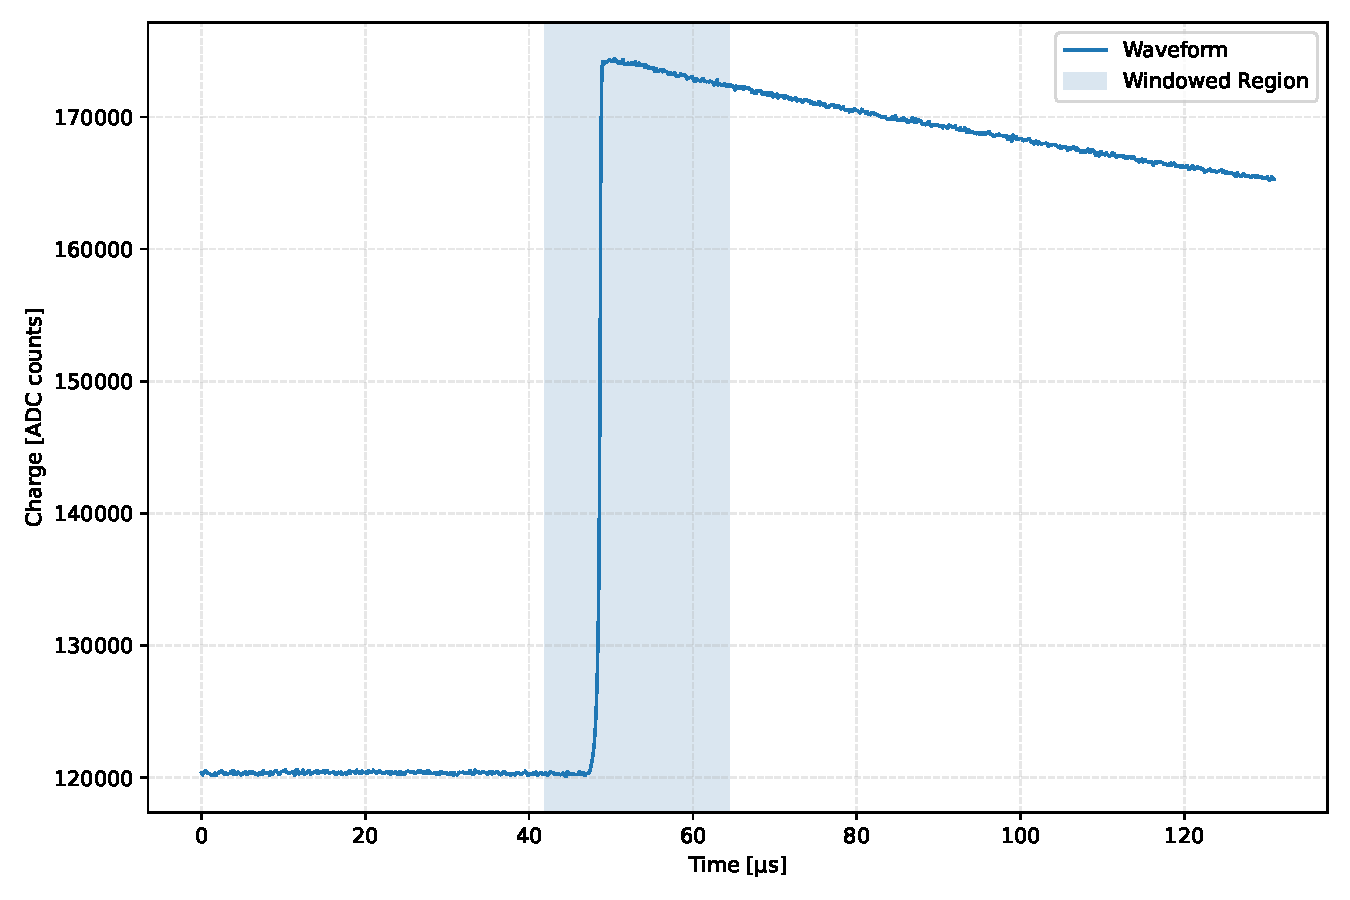
\includegraphics[width=\linewidth]{plots/wf_vs_windowed_wf.pdf}
    \caption{Example of a raw waveform from the DAQ. The windowing region is highlighted.}
    \label{fig:wf-windowing}
\end{wrapfigure}
In order to optimise data transfer and data processing, raw digitised traces are divided into two traces during the conversion from the \ac{ORCA} software to the \ac{LGDO}\footnote{\ac{LGDO} is a custom Python-based data format built by the LEGEND collaboration.} format.
For applications that do not require maximum timing resolution, such as energy reconstruction, the traces are down-sampled by summing 8 consecutive samples. This process results in a final compressed waveform of 1024 samples with a time bin width of 128 ns. Conversely, analyses like \ac{PSD} strictly require high timing resolution to resolve the signal leading edge. Therefore, a second trace is generated at the full sampling frequency, but it is restricted to a narrow window of 1400 samples (corresponding to approximately 22 $\mu$s) centered around the signal rise.  \cite{LEGEND:GeDet}\\
An example of said method is shown in Fig. \ref{fig:wf-windowing}.


\subsubsection{Data structure of the LEGEND-200 phase}
\label{subsubsec:data-structureL200}
LEGEND data are acquired in three possible modalities:
\begin{itemize}
    \item \textbf{Physics data (\texttt{phy})}: these are the data on which the physics case study is based. Signal waveforms of all the detectors in the apparatus (\ac{hpge}, \ac{lar}, and muon veto) are recorded and stored when an event is triggered by a germanium detector.
    \item \textbf{Calibration data (\texttt{cal})}: ${}^{228}$Th sources are lowered into the \ac{lar} cryostat next to the \ac{hpge} detectors to provide energy calibration data from the known $\gamma$ peaks of the Thorium decay chain (visibile in Fig. \ref{fig:decayTh228}). In this case the \ac{lar} instrumentation is turned off and each detector triggers individually.
    \item \textbf{Special calibrations or tests}: such data include different procedures to characterise the \ac{lar} instrumentation or to check the electronics for the acquisition.
\end{itemize}

Data are firstly organised in \textbf{\textit{runs}}, i.e. a 7-day data taking that starts with a calibration phase of few hours. A run is split into different files each of them characterised by the specific timestamp of the starting point. Runs are grouped in \textbf{\textit{periods}}, that are a collection of several runs sharing the same stable hardware instrumentation. Periods are then organised into \textbf{\textit{partitions}}. 

The raw data files output by the DAQ system in the ORCA format undergo a structured processing pipeline in \texttt{python} using the \texttt{pygama} library \cite{pygama}, generating distinct data tiers that correspond to the specific level of processing achieved. Said tiers are
\begin{itemize}
    \item \texttt{raw}: this is a simple conversion of the ORCA DAQ file to the LEGEND-custom \texttt{hdf5}-based data format called \texttt{lh5}. 
    During this stage, the overall data volume is effectively mitigated by partitioning the waveforms: a fully sampled waveform is preserved strictly around the leading edge, while a pre-summed waveform is retained for the complete trace. 
    Additionally, for physics runs (\texttt{phy} files), a subsequent blinding procedure is applied. Any event featuring an energy deposition of $(2039 \pm 25)$~keV---as preliminarily estimated by the DAQ software and stored in the \texttt{daqenergy} field---is systematically excluded. This specific energy window encompasses the \ac{ROI} around the $Q_{\beta\beta}$-value of the $^{76}\mathrm{Ge}$ neutrinoless double beta decay ($0\nu\beta\beta$). Hiding these data is a fundamental requirement for a blind analysis, preventing any unintended human bias while tuning the analysis cuts. To preserve synchronization and ensure that table lengths remain identical across all channels, the entire multi-channel event is discarded rather than just the single triggering channel;
    \item \texttt{tcm}: in order to reconstruct a complex event shared by multiple detectors it is crucial to know how to group together channels in which the event occur within a specific time window. This information is stored in the Time Coincidence Map files of the \texttt{tcm} tier;
    \item \texttt{dsp}: the low level signal processing routines run to extract observables such as the energy, the drift time and \ac{PSD} variables. Some of the parameters for the filters run are first optimised on calibration (\texttt{cal}) data and then passed to physics (\texttt{phy}) data to improve energy resolution;
    \item \texttt{hit}: similarly to \texttt{dsp}, parameters for the \texttt{hit} tier are first computed on calibration data. These calibrations are then applied to the parameters extracted at the \texttt{dsp} stage to define the energy in keV and the PSD classification of events;
    \item \texttt{evt}: channels in this tier are brought together exploiting the \texttt{tcm} tier in order to get a final event;
    \item \texttt{skm}: this tier is just a skimming of the event files to remove uninteresting events.
\end{itemize} 
Specific partition tiers, such as \texttt{psp} (partition \texttt{dsp}), \texttt{pht} (partition \texttt{hit}), and \texttt{pep} (partition \texttt{evt}), share the identical data structure of the standard tiers, yet their processing parameters are optimised over the entire data partition.


\subsection{Calibration data}
The analysis presented in this work is based on raw windowed waveforms, i.e. the ones for \ac{PSD}, from the \texttt{raw} tier, energy and \ac{AE}\footnote{This \ac{PSD} parameter and how it is computed will be explained in-depth at the end of this chapter in Sec. \ref{sec:traditionalPSD}.} values from the \texttt{pht} tier and rise times from the \texttt{psp} tire, both belonging to the calibration part of the \textit{prl25}\footnote{The \textit{prl25} partition corresponds to the dataset featured in the September 2025 \textit{Physical Review Letters} publication \cite{L200-sep25}.} partition. All operational runs from period \textit{p03} through \textit{p09} were utilised. Henceforth, the term dataset will be used to refer to all the runs from these periods.
Settled these premises, it is useful to analyse some aspects of said calibration dataset that will be more than crucial for the purpose of this work\footnote{Details about the number of events, their selection, cleaning and filtering will be discussed further in Chapter \ref{chapter:ML-PSD}}.

Energy calibration is performed using Thorium-228 sources with low neutron emission. The sources are inserted in the LAr cryostat through four calibration systems, each moving four ${}^{228}$Th sources of about 5 kBq activity per source, situated at different heights for homogeneous event distribution (\cite{L200:calibration}, \cite{LEGEND:GeDet}). The decay chain of such isotope is shown in Fig. \ref{fig:decayTh228} while the energy spectrum of $\gamma$-rays emitted as a consequence of the decays are visible in Fig. \ref{fig:TlBi-spectrum}. It is evident that we can distinguish several peaks: the ones we are focusing on are listed in Table \ref{tab:emission-peaks}.

\begin{figure}[H]
    \centering
    \begin{minipage}[t]{0.3\textwidth}
        \vspace{0pt} % Forza l'allineamento al margine superiore
        \centering
        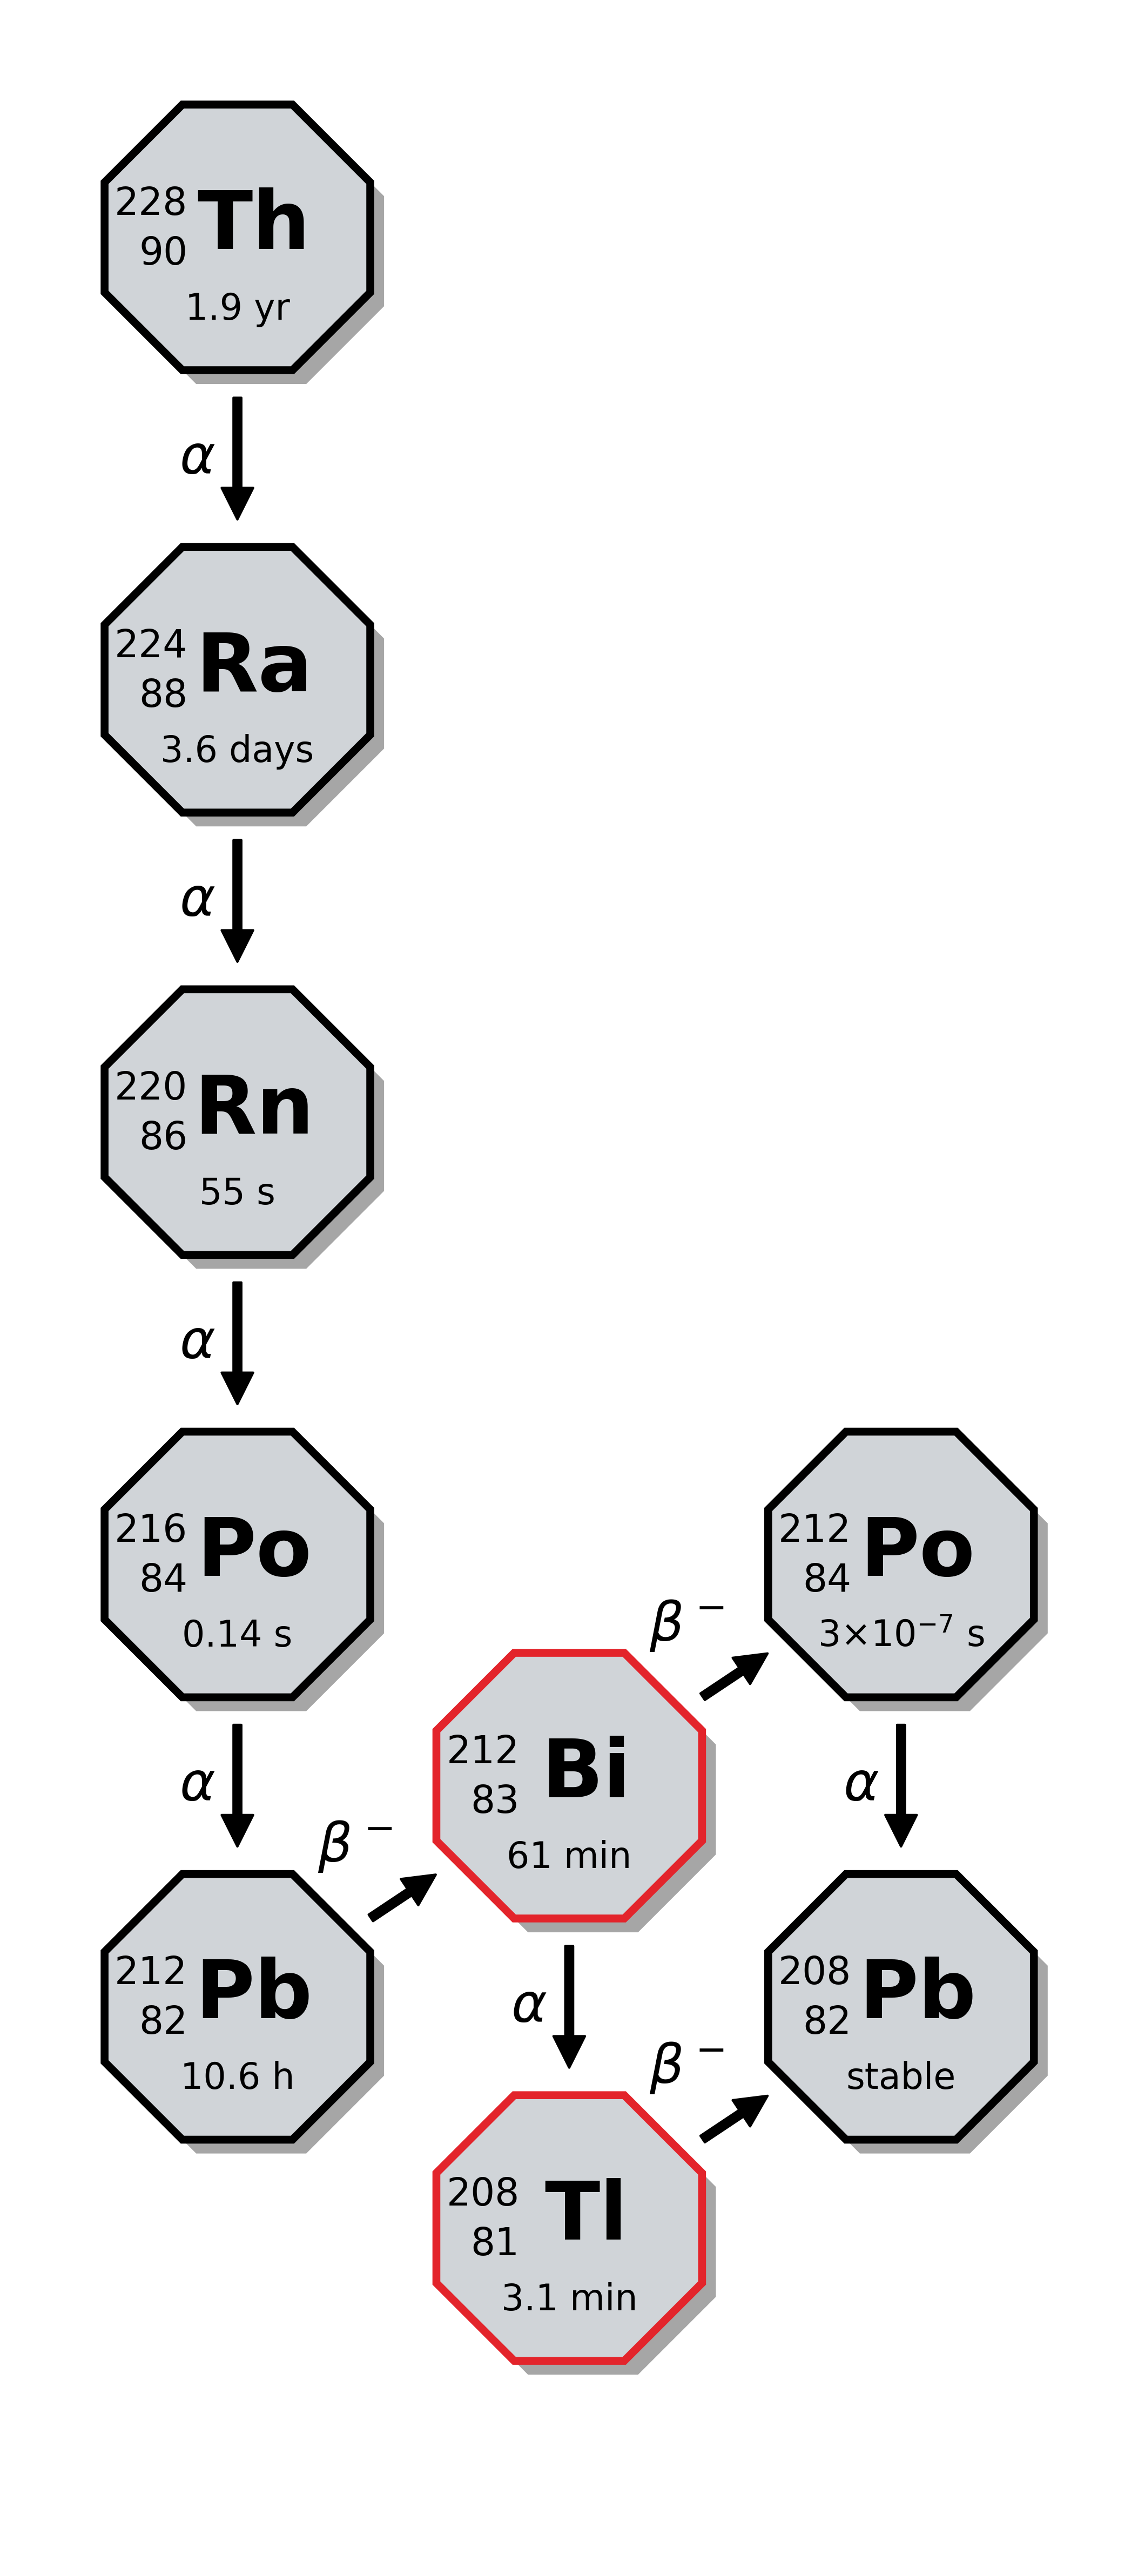
\includegraphics[width=\linewidth]{figures/catena_decadimento_Th228.png}
        \caption{Decay chain of the ${}^{228}$Th source. Custom plot with data taken from \cite{Th228chain}.}
        \label{fig:decayTh228}
    \end{minipage}
    \hfill 
    \begin{minipage}[t]{0.65\textwidth}
        \vspace{0pt} % Forza l'allineamento al margine superiore
        \centering

        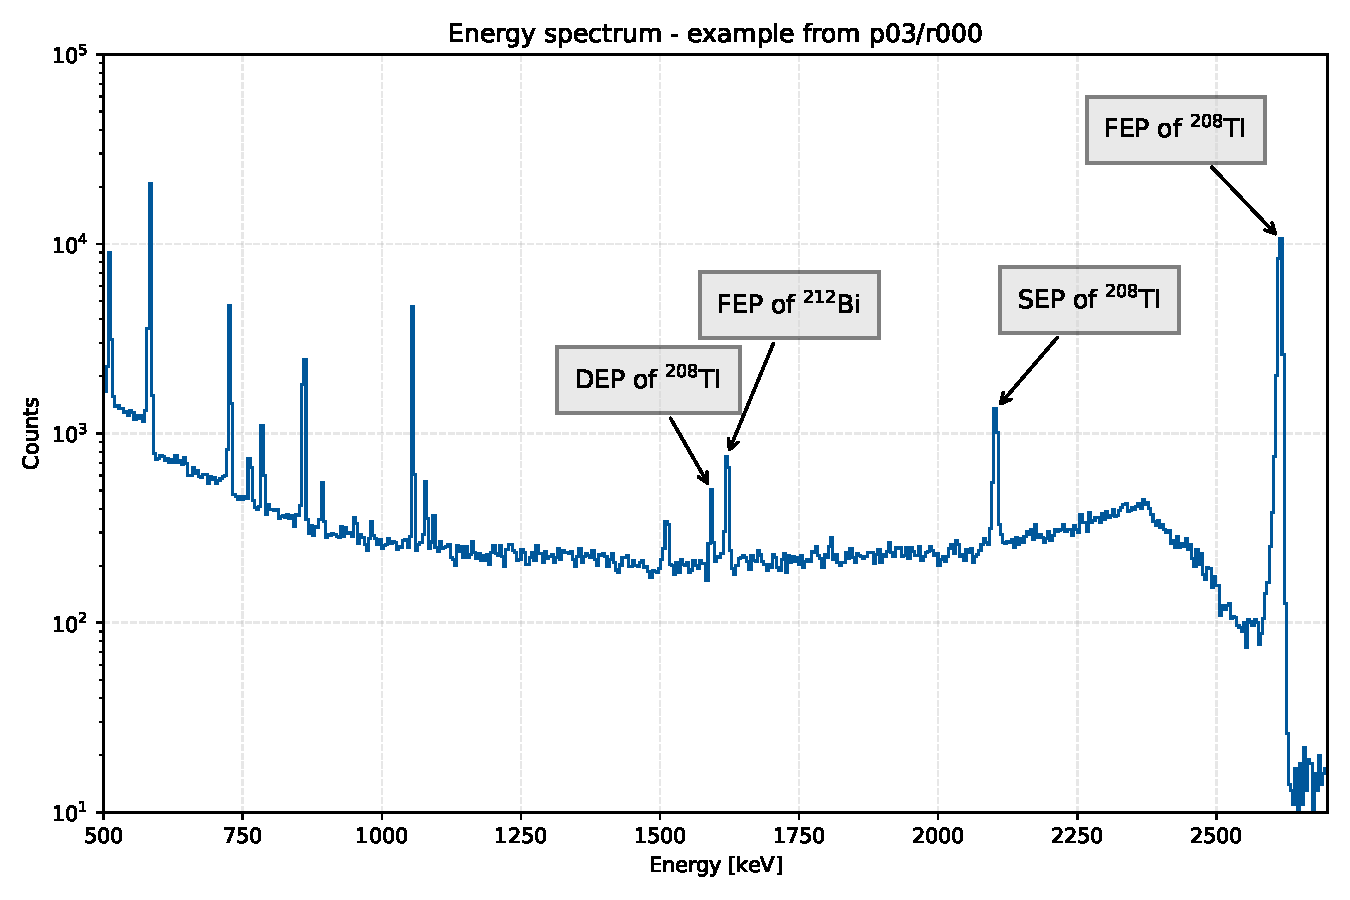
\includegraphics[width=\linewidth]{plots/energy_spectrum-example.pdf}
        \caption{Example of the energy spectrum recorded in a calibration run. Peaks listed in Tab \ref{tab:emission-peaks} are highlighted. Data for this example plot are from run \textit{r000} of period \textit{p03}.}
        \label{fig:TlBi-spectrum}
        
        \vspace{1.0em}

        \begin{tabular}{ccccc}
            \toprule
            \textbf{Isotope} && \textbf{Peak} && \textbf{Energy [keV]} \\
            \midrule
            $^{208}$Tl && FEP && 2614.511 (10) \\
            $^{208}$Tl && SEP && 2103.511 (10) \\
            $^{208}$Tl && DEP && 1592.511 (10) \\
            $^{212}$Bi && FEP && 1620.738 (10) \\
            \bottomrule
        \end{tabular}
        \captionof{table}{Prominent $\gamma$-ray peaks from the $^{228}$Th decay chain used for energy calibration. Data are taken from \cite{LNHB}.}
        \label{tab:emission-peaks}
    \end{minipage}
\end{figure}

\ac{DEP}, \ac{SEP} and \ac{FEP} of Thallium-208 correspond to distinct interaction mechanisms following a pair production event inside the detector, as illustrated in Fig.~\ref{fig:dep-sep}. 
\begin{figure}[H]
    \centering
    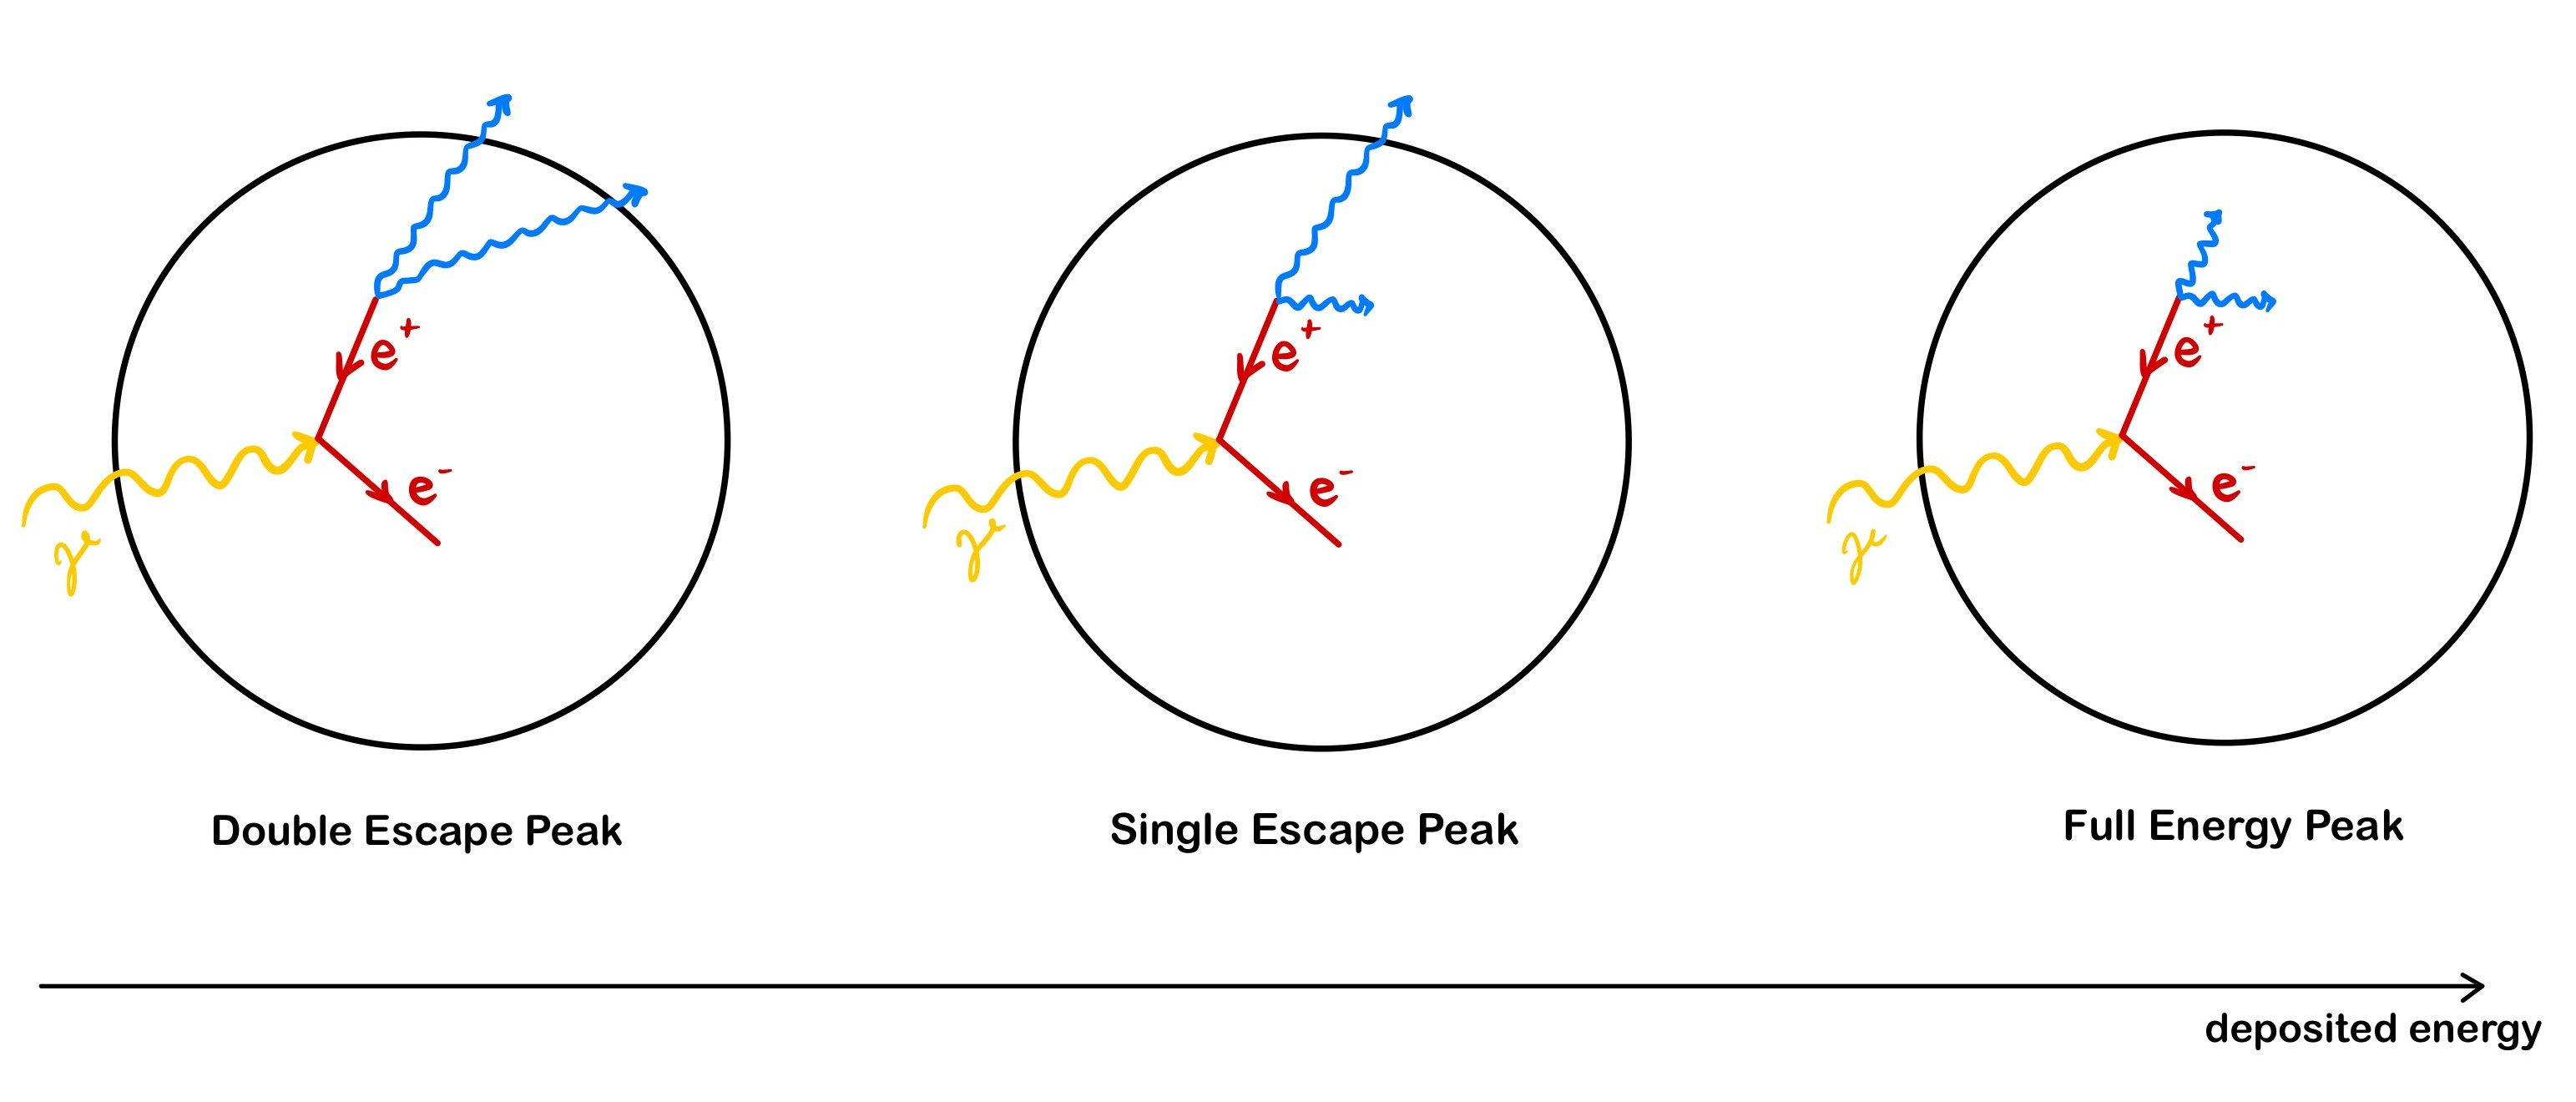
\includegraphics[width=0.9\textwidth]{figures/DEP-SEP-FEP.jpg} 
    \caption{Different outcomes after a gamma interaction in the detector volume, delimited in black.\\A detailed description of the phenomena illustrated is given in the text.}
    \label{fig:dep-sep}
\end{figure}
Specifically, a \ac{DEP} event occurs when a high-energy $\gamma$ ray undergoes pair production, and both resulting 511 keV annihilation photons of the positron escape the active detector volume without further interaction. Consequently, the energy deposition is highly localised, yielding a simple and temporally narrow pulse waveform associated to \ac{SSE}.
Conversely, a \ac{SEP} event arises when only one of the two annihilation photons escapes, while the second photon re-interacts and deposits its energy elsewhere within the detector volume. This spatial separation introduces a temporal spread, resulting in a more complex waveform structure. Furthermore, events contributing to the \ac{FEP}, both of Thallium-208 and of Bismuth-212, typically involve multiple Compton scattering interactions prior to complete absorption, yielding an even more intricate pulse shape. These last two peaks are typical \ac{MSE}.



From now on, we are interested in considering the two peaks corresponding to the \ac{DEP} of ${}^{208}$Tl and the \ac{FEP} of ${}^{212}$Bi: hey are very close to each other in energy, as stated in Table \ref{tab:emission-peaks}, but are produced in different mechanisms consequently producing different signals in \ac{hpge} detectors, respectively \ac{SSE} and \ac{MSE}. This is significant in the context of our research since what we really want to investigate and discriminate is the shape of the waveform of specific signals; therefore any energy dependence in such shape is to be eliminated. In this perspective, selecting events with comparable energies isolates the waveform from energy-induced variations, allowing us to rely solely on the time evolution of its shape. 

Nonetheless it is important to stress that this \ac{SSE} and \ac{MSE} labelling is statistical rather than exact event by event. As it is clear in Fig. \ref{fig:TlBi-spectrum} the two peaks we are considering lie over a continuous background . Therefore when considering the \ac{DEP} peak, a fraction of events with a \ac{MSE} topology arising from multiple Compton scattering are considered as well; viceversa the \ac{FEP} peak may contain a fraction of \ac{SSE}. However since these peaks significantly exceed the level of the background they are statistically dominated by the \ac{SSE} topology and \ac{MSE} respectively. Therefore, whenever we refer to \ac{SSE} and \ac{MSE} what we mean is that statistically they actually are so. 
% Said considerations are clearly a limitation both for traditional classifiers and machine learning ones relying on pulse shapes.


\newpage
\section{Traditional \ac{PSD}}
\label{sec:traditionalPSD}
Pulse shape discrimination \ac{PSD} is employed in the LEGEND program with several purposes in order to enhance the signal-like events with respect to the background ones. Two main parameters are employed in this procedure: the \ac{LQ} and the \ac{AE}. 

The first one is a easure of the \textit{slowness} of the final 20\% of charge carriers for an event. It is determined by calculating the area above the rising edge of the waveform after it reaches the 80\% of its maximum. DSince surface events (both alpha and beta) tipically manifest a slow-charge trend with a incomplete charge collection as a consequence, \ac{LQ} is expected to be a powerful discriminator against these events, which constitute a part of the background (see Sec.~\ref{sec:background}). 

On the other hand, \ac{AE} represents the main basis on which \ac{MSE} rejection relies. It is computed as the ratio between the amplitude of the first peak of the current signal (obtained from the raw charge signal via time derivative) and the energy of that event. In principle, if we consdier a \ac{SSE} and a \ac{MSE} at the very same energy, the \ac{AE} ratio will be smaller for a \ac{MSE} that exhibits many current peaks lower than the one of the \ac{SSE}. 
Figure \ref{fig:AoE_distribution} makes it evident that different physical processes are correlated with different \ac{AE} distributions, therefore a proper selection of this value enable to distinguish signal-like events from background-like ones.

\begin{figure}[H]
    \centering
    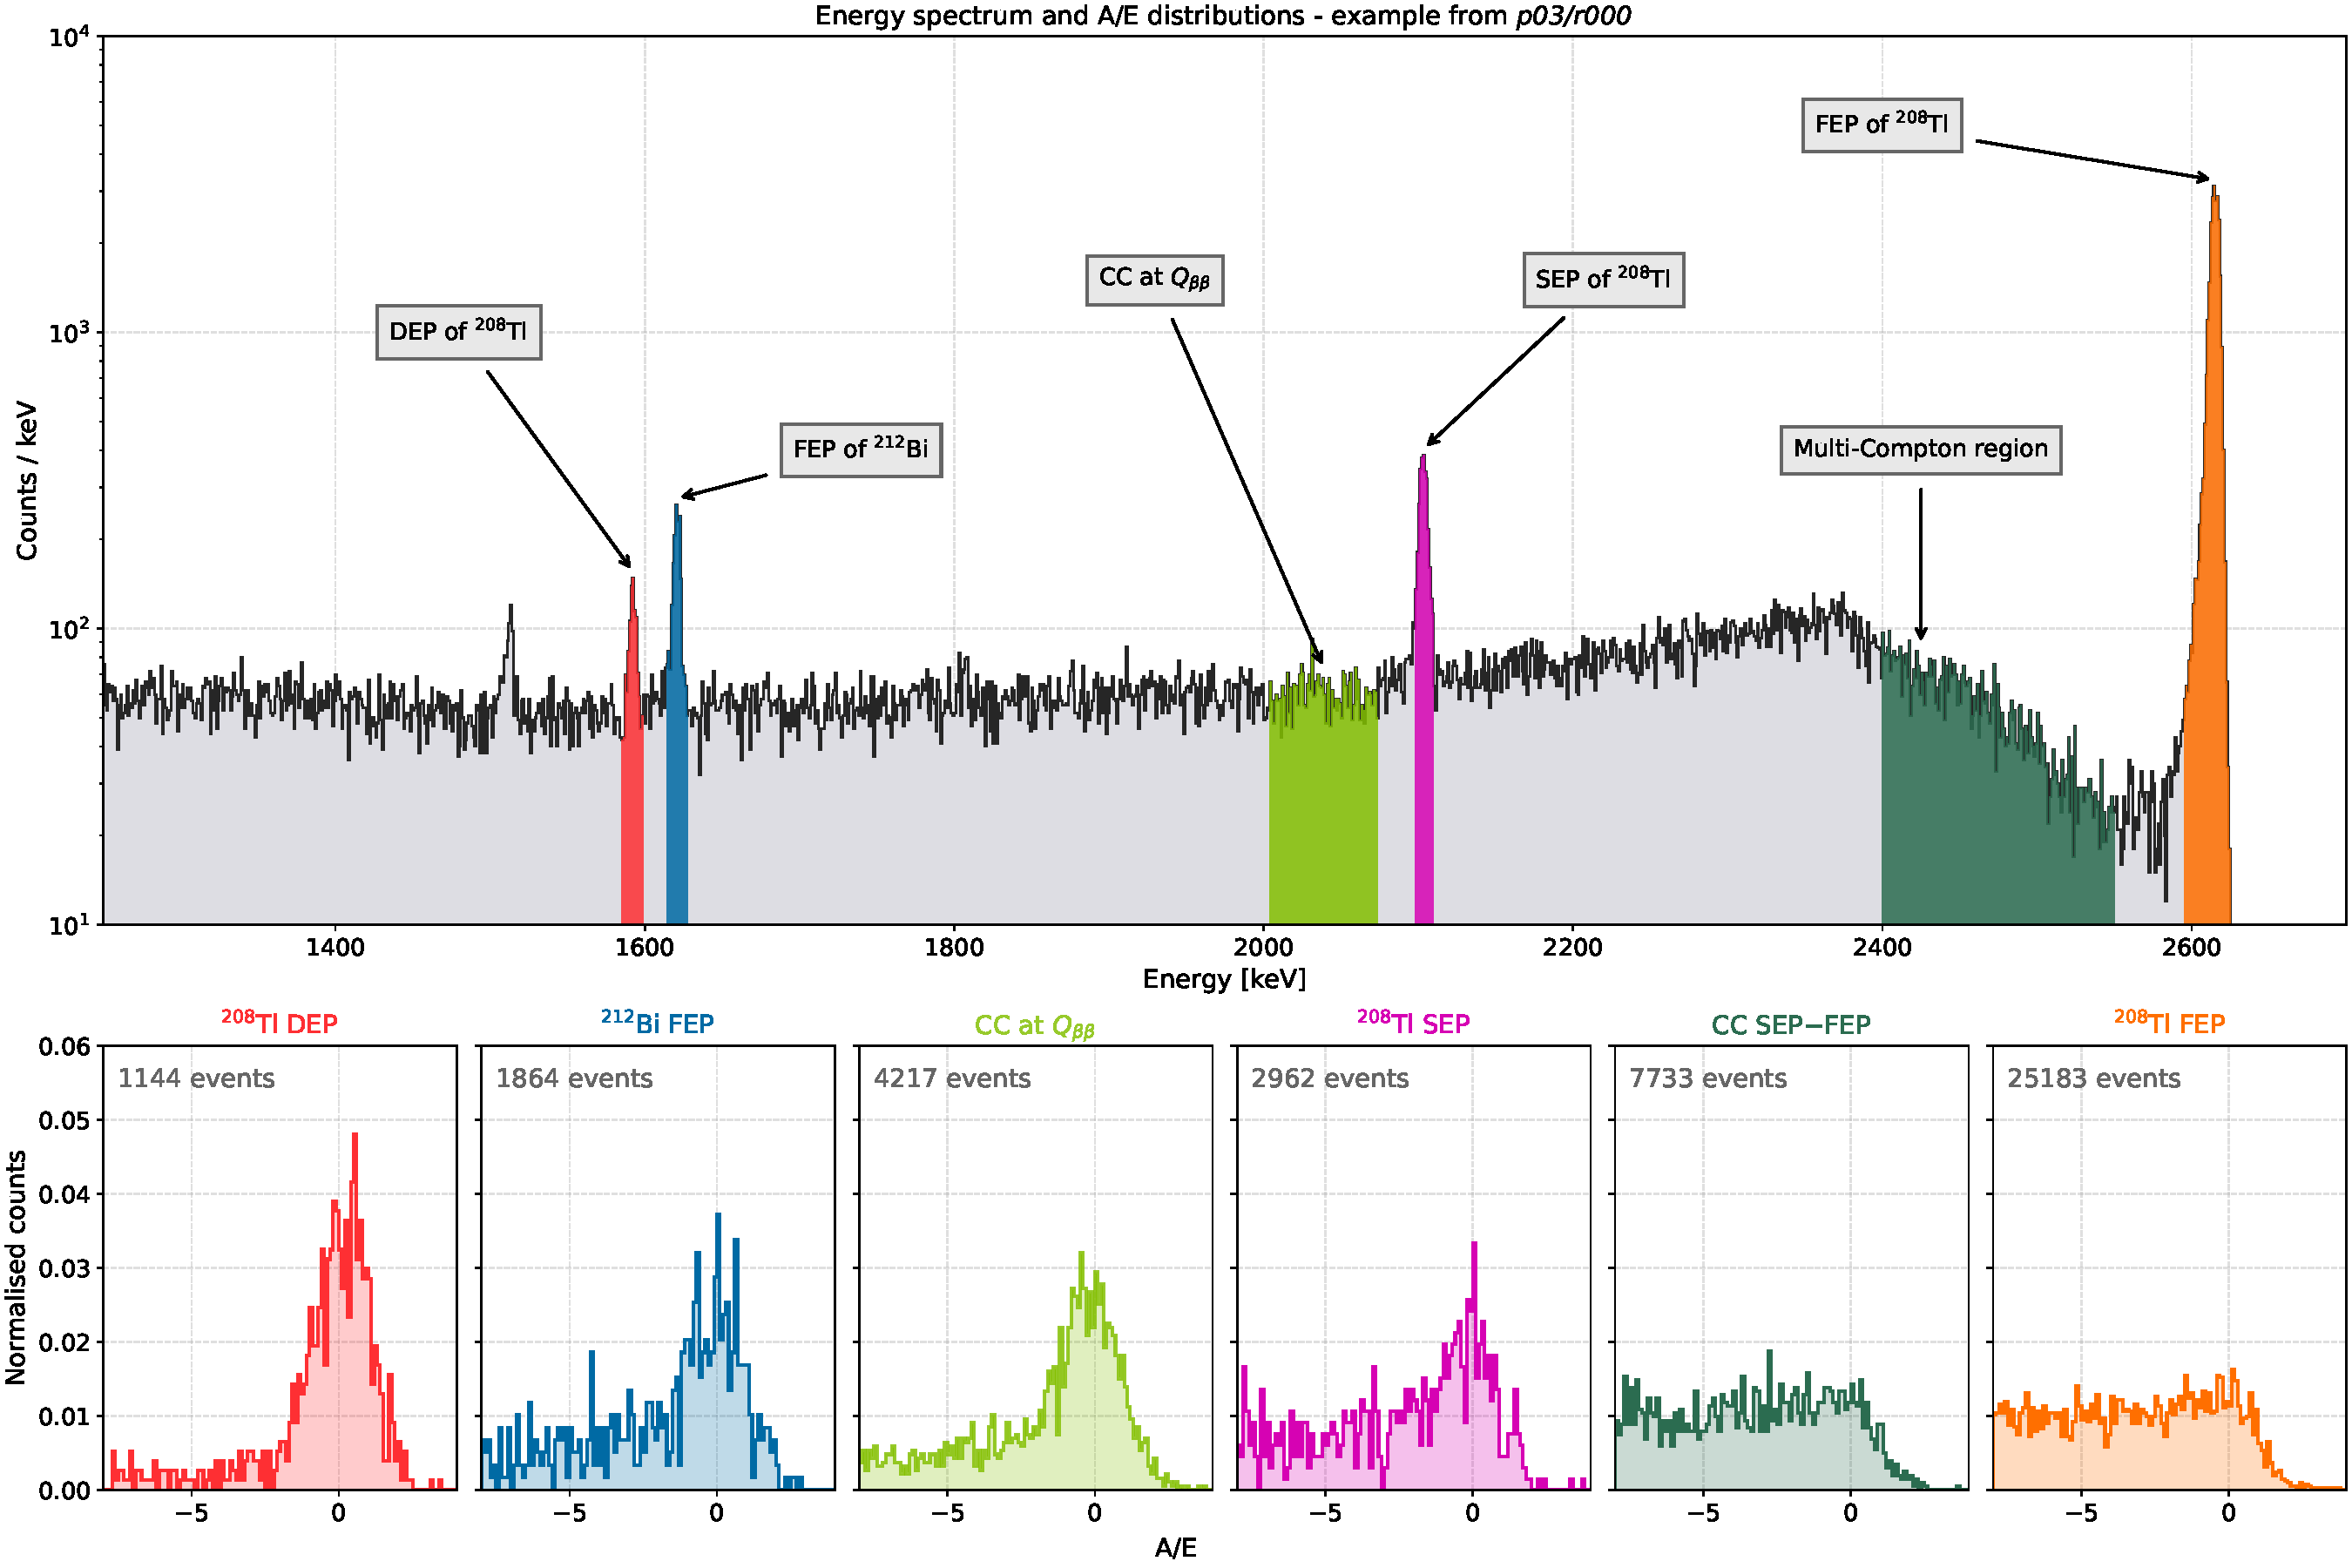
\includegraphics[width=\textwidth]{plots/energy_spectrum_and_aoe-example.pdf}
    \caption{\ac{AE} distributions in different ranges of the calibration spectrum. Data are from run \textit{r000} of period \textit{p03}.}
    \label{fig:AoE_distribution}
\end{figure}



Figure~\ref{fig:distribution-AoE_prl25} presents the \ac{AE} cut for the calibration data of \textit{prl25} in the $1550-1650$ keV energy range. Because of physics and computational reasons only said data have been employed for this work, as will be discussed in Sec.~\ref{sec:data-cleaning}. This \ac{PSD} cut will be the benchmark for all the others that have been implemented in this work and will be presented in Chapter \ref{chapter:ML-PSD}
\begin{figure}[H]
    \centering
    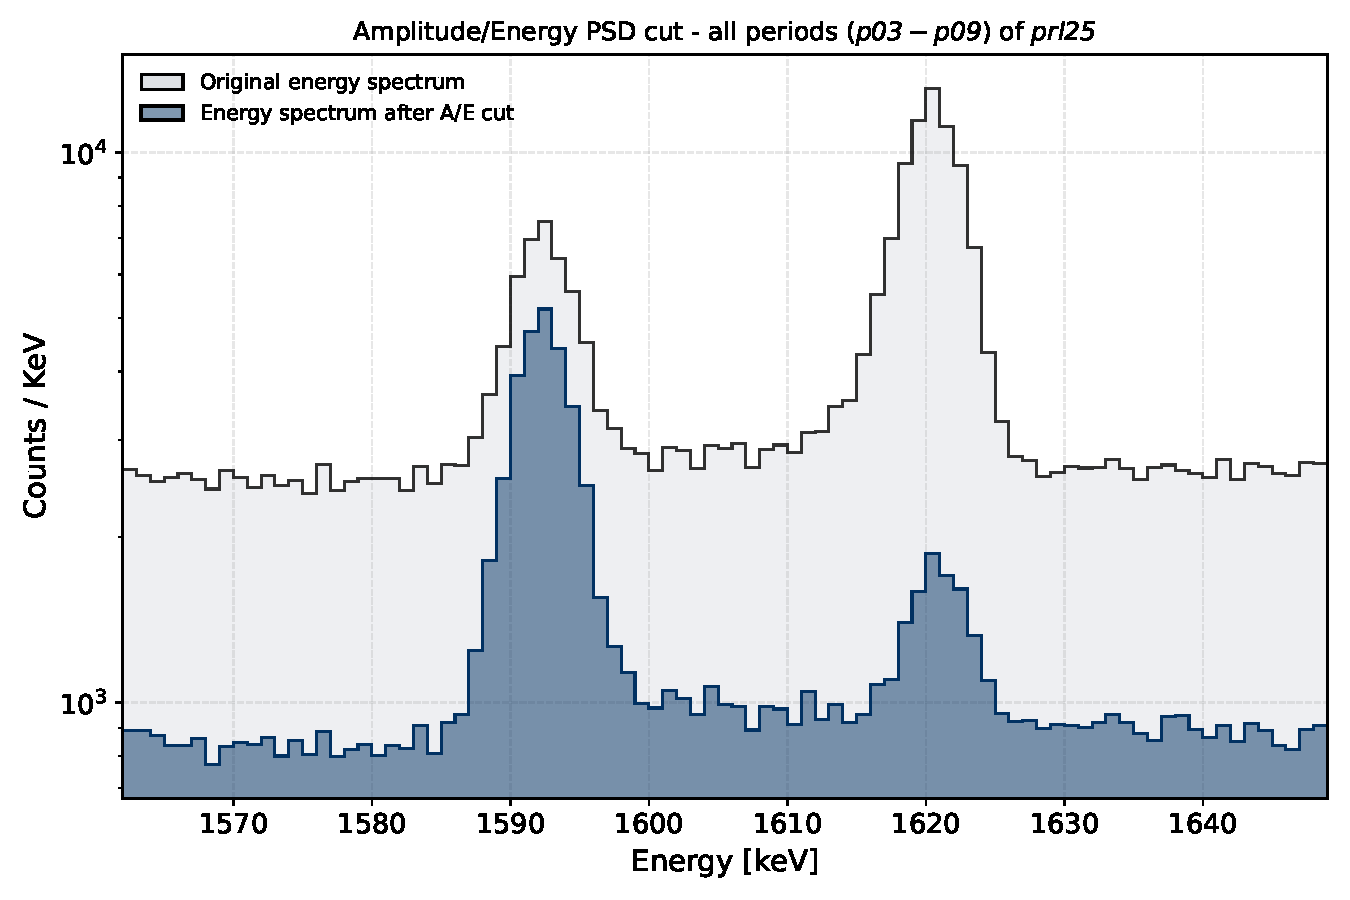
\includegraphics[width=\textwidth]{plots/energy_specrum-prl25-AoE_cut.pdf}
    \caption{Windowed energy spectrum before (gray) and after (blue) the A/E cut. The cut is tuned in order have a survival fraction in the \ac{DEP} of 90\%.}
    \label{fig:distribution-AoE_prl25}
\end{figure}



